\documentclass[12pt,letter]{article}
 \linespread{1.25}
\usepackage[left=1in,right=1in,top=1in,bottom=1in]{geometry}
\usepackage{amsmath}
\usepackage{pdflscape}
\usepackage{amsfonts}
\usepackage{amssymb}
\usepackage{graphicx}
\usepackage{caption}
\usepackage{multicol}
\usepackage{microtype}
\usepackage{euscript}
\usepackage{epsfig}
\usepackage{verbatim}
\usepackage{epstopdf}
\usepackage{mathrsfs}
\usepackage{tikz}
\newcommand{\hypo}{\mathcal{H}}            
\bibliographystyle{ieeetr}

\usepackage[flushleft]{threeparttable}

\usetikzlibrary{shapes,arrows}
\usetikzlibrary{positioning}
\tikzstyle{block} = [rectangle, draw, rounded corners]
\tikzstyle{line} = [draw, -latex']



%\usepackage[cp1251]{inputenc}
\usepackage[english]{babel} 
\DeclareMathOperator{\rank}{rank}
\newcommand*{\hm}[1]{#1\nobreak\discretionary{}
            {\hbox{$\mathsurround=0pt #1$}}{}}

            \def\onepc{$^{\ast\ast}$} \def\fivepc{$^{\ast}$}
\def\tenpc{$^{\dag}$}
\def\legend{\multicolumn{4}{l}{\footnotesize{Significance levels
:\hspace{1em} $\dag$ : 10\% \hspace{1em}
$\ast$ : 5\% \hspace{1em} $\ast\ast$ : 1\% \normalsize}}}


\newcommand{\bs}[1]{\boldsymbol{#1}}  
\newcommand{\bsA}{\boldsymbol{A}}

%\setstretch{1}                         
\flushbottom                            
\righthyphenmin=2                      
\pagestyle{plain}                       
%\settimeformat{hhmmsstime}  
\widowpenalty=300                   
\clubpenalty=3000                     
\setlength{\parindent}{0em}           
\setlength{\topsep}{0pt}              
\usepackage[pdftex,unicode,colorlinks=true,urlcolor=blue]{hyperref}
\usepackage{bbm}
\renewcommand{\emptyset}{\varnothing}

\setlength{\parskip}{0.5\baselineskip plus2pt minus2pt}

\newcommand{\e}{\varepsilon}
\DeclareMathOperator*{\Argmax}{\mathrm{Argmax}}
\DeclareMathOperator*{\Argmin}{\mathrm{Argmin}}
\DeclareMathOperator*{\argmax}{\mathrm{arg\,max}}
\DeclareMathOperator*{\argmin}{\mathrm{argmin}}

\newcommand{\blp}{\mathrm{BLP}}
\DeclareMathOperator*{\plim}{\mathrm{plim}}
\DeclareMathOperator{\Max}{\mathrm{Max}}
\newcommand{\R}{\mathbb{R}}
\newcommand{\Y}{\mathcal{Y}}
\newcommand{\Z}{\mathcal{Z}}
\renewcommand{\geqslant}{\geq}
\renewcommand{\leqslant}{\leq}
\newcommand{\p}{\bs p}
\newcommand{\y}{\bs y}
\def\dd#1#2{\frac{\partial#1}{\partial#2}}

\renewcommand{\emptyset}{\varnothing}


\DeclareMathOperator{\tr}{\mathrm{tr}}

\newcommand{\bb}{\bs \beta}
\newcommand{\X}{\bs X}
\DeclareMathOperator{\E}{\mathbb{E}}
\DeclareMathOperator{\PP}{\mathbb{P}}
\DeclareMathOperator{\V}{\mathbb{V}}
\DeclareMathOperator{\CM}{\mathbb{C}}
\renewcommand{\C}{\CM}
\DeclareMathOperator{\var}{\mathrm{var}}
\DeclareMathOperator{\cov}{\mathrm{cov}}
\DeclareMathOperator{\corr}{\mathrm{corr}}
\DeclareMathOperator{\MSE}{\mathrm{MSE}}
\DeclareMathOperator{\Bias}{\mathrm{Bias}}
\renewcommand{\P}{\PP}
\newcommand{\dsim}{\stackrel{d}{\sim}}
\newcommand{\hn}{\mathcal{H}_0}
\newcommand{\ha}{\mathcal{H}_a}
\newcommand{\thetab}{\bs \theta}
\newcommand{\pv}{\text{P-value}}
\newcommand{\N}{\mathcal{N}}
\newcommand{\MLE}{\scriptscriptstyle MLE}
\newcommand{\LR}{\mathrm{LR}}
\newcommand{\I}{\mathbb{I}}
\newcommand{\sumin}{\sum\limits_{i=1}^n}
\newcommand{\sumti}{\sum\limits_{t=0}^\infty}
\newcommand{\hbeta}{\hat{\beta}}
\newcommand{\halpha}{\hat{\alpha}}
\newcommand{\hsigma}{\hat{\sigma}}
\newcommand{\hvar}{\widehat{\var}}
\newcommand{\hcov}{\widehat{\cov}}
\newcommand{\Q}{\mathbb{Q}}



\newcommand{\pconv}{\xrightarrow{ \ p \ }}
\newcommand{\dconv}{\xrightarrow{ \ d \ }}
\newcommand{\asconv}{\xrightarrow{ \ a.s. \ }}
\newcommand{\msconv}{\xrightarrow{ \ m.s. \ }}

\newcommand{\pic}[4][h!]{\begin{figure}[#1]


\begin{center}\includegraphics[width=#2cm]{#3}\caption{#4\label{#3}}\end{center}
\end{figure}}

%outtex
\def\onepc{$^{\ast\ast}$} \def\fivepc{$^{\ast}$}
\def\tenpc{$^{\dag}$}
\def\legend{\multicolumn{4}{l}{\footnotesize{Significance levels
:\hspace{1em} $\dag$ : 10\% \hspace{1em}
$\ast$ : 5\% \hspace{1em} $\ast\ast$ : 1\% \normalsize}}}
%end outtex

%\bibliographystyle{ieeetr}

\newcommand{\laseq}{\stackrel{\lambda\text{-a.e.}}{=}}
\renewcommand{\d}{\underline}
\renewcommand{\u}{\overline}
\newcommand{\td}{\underline{\theta}}
\newcommand{\tu}{\overline{\theta}}
%\renewcommand{\theenumi}{\alph{enumi}}
%\renewcommand{\labelenumi}{(\theenumi)}
%\renewcommand{\theenumii}{\roman{enumii}}
%\renewcommand{\labelenumii}{\theenumii.}
%\renewcommand{\theenumiii}{\arabic{enumiii}}
%\renewcommand{\labelenumiii}{\theenumiii.}
%\renewcommand{\epsilon}{\varepsilon}
\newcommand{\hneq}{\stackrel{\hn}{=}}
\newcommand{\deq}{\stackrel{d}{=}}


\clubpenalty=10000
\widowpenalty=10000
\begin{document}

\title{The Economics of Shotgun Marriage}
\author{Egor Kozlov\thanks{Economics Department, Northwestern University, egorkozlov2020@u.northwestern.edu. I thank my advisors Matthias Doepke, Martí Mestieri, and Alessandra Voena, for a fantastic amount of help and support as part of my dissertation committee. I thank my colleagues Jane Olmstead-Rumsey, Kristina Manysheva, Bence Bardoczy, Stephanie Johnson, and Gabriela Cugat, as well as all the participants of Macro Lunch at Northwestern, Midwest Macro Meetings, and H2D2 Research Day for lots of helpful comments. I owe special thanks to Fabio Blasutto for tons of help with both technical and substantial parts during his stay at Northwestern and after.}\\[1.5cm] Job Market Paper \\ \href{http://egorkozlov.link/jmp-kozlov.pdf}{Latest version available here}}
\maketitle

\begin{abstract}
Many couples marry either just before or soon after they have their first child. I show that married couples who have the first child before or in the year of marriage (kids-first) divorce around twice more often than those having their first kids in the year following their marriage or later (marriage-first). Various well-known determinants of divorce do not explain this difference. I show that it is consistent with a simple setup where people choose whether to marry based on their potential relationship quality. Unplanned pregnancies can affect their decisions as women face a risk of raising the child alone. I build and estimate a lifecycle model capable of quantifying this selection pattern. Through the model's lens, around forty percent of kids-first couples marry \textit{because} they have a child. However, a natural response of forcing fathers to pay child support has a very mild impact on these couples' marriage and divorce decisions. In contrast, improving people's ability to control their fertility provides the highest return. For existing marriages, delaying or limiting fertility is a response to the risk of divorce.
\end{abstract}

\newpage
\section{Introduction}
Marriage is associated with a range of desirable outcomes. Controlling for age and education, married couples are wealthier on a per-capita basis than never married or divorced. Marriage provides spousal insurance and efficient cooperation within the household. The benefits are especially apparent when it comes to children: married two-parent families are considered the best in terms of early and adult-life outcomes of children relative to never married or divorced parents (Chetty, Hendren, 2018\nocite{chetty2018impacts}; Ginther, Pollak, 2004\nocite{ginther2004family}). It is common, especially among conservative voices, to refer to marriage as ``America's strongest anti-poverty weapon.''\footnote{See congressman Ted Budd \href{https://www.dailysignal.com/2020/02/24/marriage-is-the-ticket-out-of-poverty/}{here}, among others.} 

Is it a good idea to make people marry more? Generally, this depends on what we believe are the \emph{causal} benefits of marriage. For sure, married people do better, but is this related to the fact they are married? A simple marginalist answer is negative: if people choose whether to marry, and marriages differ in quality, than making people marry more means allowing for lower quality marriages with the lowest benefit from them to be created. The competitive market may just be not the right setup to think about this. Still, marriages are not created equal, and some marginal partnerships can be very similar to singlehood. 

In this paper I argue that the contrast between marriage and singlehood leaves out an important distinction. Some marriages follow the birth of the first child; others take place before the couple has children. Formally, I define ``kids first'' marriages as marriages for which the first child was born before or at the year of the marriage and ``marriage first'' as those marriages for which the childbirth happened at least in the following year. The former group includes what is traditionally referred to as a ``shotgun marriage'' --- a marriage that occurs when a bride is pregnant. Like shotgun marriages, the kids-first marriages suggest that an unintended pregnancy contributed to the decision to get married. And as I show later, the kids-first couples are marginal in terms of responses to the environment: their creation and dissolution are sensitive to the economic situation and policies.

I document that among women 21--40 in the US, 14\% of kids-first unions end in divorce within five years, as opposed to 5\% for marriage-first. Most of this difference cannot be explained by various ways of controlling for age, demographics, education, and income. This pattern is robust to different choices of time horizons and measures of divorce. Perhaps more surprising, the difference is the largest for the educated people, yet the share of the kids-first marriages is lower for them. Namely, kids-first college graduates divorce more than three times more often than the marriage-first, as opposed to less than 1.5 for those who finished only a high school. A similar pattern applies if I separate early and late births: although women giving the first birth before 25 are more likely to be in a kids-first marriage, the underperformance of such marriages is relatively milder than for those with later births.

% Need for the model.
Even though the data pattern is evident, the lack of exogenous variation in marriage timing does not explain why people experience such different outcomes and the channels generating this difference. In a more narrow sense, if we believe that the kids-first marriages have worse unobservable quality causing them to be less stable, studying policy and welfare questions require understanding the magnitudes of these quality differences. I develop a quantitative model that can, essentially, map the differences in the divorce rates into marriage quality differences. 

My structural approach helps to answer several questions. First, what explains the difference in performance between the kids-first and other marriages? Second, what part of the value of marriage is generated by having children together? Third, what is the role of child support and related policies in the creation and dissolution of the shotgun marriages and in shaping the number of single mothers in the economy in general?

The model is based on a dynamic limited commitment framework (Kocherlakota 1996\nocite{kocherlakota1996implications}, Ligon, Thomas, Worrall, 2000\nocite{ligon2000mutual}, Marcet, Marimon 2019\nocite{marcet2019recursive}),  in which I endogenize marriage, divorce, and fertility choice. People are heterogeneous with respect to age, labor productivity, and savings. In a random search spirit, they randomly meet potential matches and form couples, which also differ in the relationship quality and relative decision power of spouses. When a couple meets, the decision power is determined by symmetric Nash Bargaining. The relationship quality --- commonly referred to as love shock --- is the crucial factor affecting people's decisions to marry. Spouses cannot commit not to divorce, so their choices are subject to the participation constraints determined dynamically based on their option to divorce and possibly find new partners. Married childless couples endogenously decide on their fertility timing; children bring utility and require both money and time.

A main driving force for the marriage timing in the model is random fertility shocks happening to the partners before making their marriage decision. When a potential couple meets, with some chance they have an unplanned child. If this happens, the couple's bargaining is affected: if the partners agree, they become a (kids-first) couple with a child; otherwise, the woman risks becoming a single mother or facing a costly pregnancy abortion, and the man loses access to the child. Relative to the regular situation, in which upon disagreement partners just wait for their new matches, this generates different selection into a marriage based on fertility timing, and the model fundamentals determine its strength and implications. In particular, the model predicts that if the unplanned pregnancy happened, some couples with inferior match quality agree to marry each other, which later generates a higher risk of divorce. The intuition for this comes from two things: people generally like the arrival of children, and being a single mother or aborting is not a desirable option.

I estimate the model parameters using a simulated method of moments, matching the established data evidence to the quantities in the simulated data. The parameters I estimate are the preference for children, household technology features, and the transition probabilities. I match several sets of moments. The most important thing is the percentage of divorced women by different durations of marriage in the kids-first and the marriage-first group. I also include the share of never-married and divorced with and without kids by age, the percentage of couples having children by the duration of their marriage, and several other things. To account for the education gradient flexibly, I perform two separate estimations on two subgroups --- college graduates and high school graduates. The model fits very well in both subgroups, with few exceptions for the high school graduates where the fit is still reasonable.

Qualitatively, the estimates indicate a significant uninsurable risk of unplanned pregnancies that people face. There are substantial differences in the probability of unplanned pregnancy between the high school and the college groups. For both of them, the risk has the monetary equivalent of several years of labor earnings. The risk is relatively larger for college. Moreover, the estimates indicate that the threshold for relationship quality that is acceptable for partners to agree to marry each other falls following the shock, leading to the creation of marriages that would not happen without an unplanned pregnancy. These marriages almost mechanically have the highest risk of divorce. Finally, following an unexpected pregnancy, the woman's outside option drops: on average, she does not want to raise the kids on her own, unless she is highly productive or has considerable savings. This drop decreases her decision power inside marriage, leading to potentially different outcomes even for couples with relatively high marriage quality.


The model provides a way to look at post-marital policies like the child support. Some women would choose not to enter marriages if they can just collect child support and raise their children as single mothers. In addition, women in existing marriages can be more tempted to leave. This can cause a response such that some marriages would not be created, and many other selection-related results. Therefore, the welfare can be affected either way. The model argues that more child support is generally welfare improving, and to some extent it is welfare improving for both men and women, so it is far from being just a redistribution. On the other hand, its effects on creation and dissolution of shotgun marriages itself is minimal, although it affects the share of single mothers by making couples divorce more and singles to abort pregnancies less often.

% Gram
More generally, the model can touch whether keeping people married is good, even though marriage is an endogenous decision. One obvious way to create more marriages is to make divorce easier! It creates more marriages and induces large welfare gains. However, the model also predicts a sizable decrease in in-marriage fertility. Shortly, those couples that stick together because there is an easy way to exit a marriage rarely have kids. Although people win from easier divorce, this does not look like a desirable outcome from the conservative view.

On the other hand, the model suggests that reducing the pressure for people to marry following an unplanned pregnancy and giving people better control over their fertility is beneficial in welfare for both parents and children. These two measures combined reduce the count of single mothers in the economy. The former is more important for the high school graduates and the latter --- for the college graduates. 

Quantitatively, more than half of college and a bit less of high-school kids-first couples marry because they had a pregnancy. Each of three factors - imperfect fertility control, social stigma against unmarried parenting, and difficult remarriage after a birth - explain one-third to one-half of excess divorces of the kids-first couples, and their interaction is non-negligible. Eliminating existing child support has minor effects on the creation of shotgun marriages, and the largest margin that it affects is the percentage of abortions. The welfare benefits of child support can go both ways. In some cases, elimination of it benefits both parents and children, together with decreasing divorce rates and single mothers' share. However, expanding child support may also be beneficial in some welfare dimensions.

My paper contributes to the literature in several ways. First, I am the first to document a strong and robust underperformance of kids-first marriages in modern US data. Second, I am the first to estimate a lifecycle model of marriage and divorce featuring a fertility choice, which is central in the model. Third, I am the first to study the interaction of creation and dissolution of shotgun marriages from public policy prospectives, which previously have been considered in isolation while being importantly related as two sources of formation of single-parent families.

I am not the first to study shotgun marriages in the literature. A seminal piece of research is Akerlof, Yellen, Katz, 1996\nocite{akerlof1996analysis}. They interpret them as commitment technology to access premarital sex and argue that contraception and abortion technologies lead to this practice's disappearance. Further, welfare expansion (Neal, 2004\nocite{neal2004relationship}) and the stock of potential partners (Chiappori, Oreffice, 2008\nocite{chiappori2008birth}) were argued to influence women's decision to enter marriages following pregnancies. However, these models are mostly of illustrative purposes. In contrast to this, my model is a quantitative study capable of delivering policy counterfactuals and welfare implications.

Empirically, Alesina, Giuliano, 2005\nocite{alesina2006divorce} have shown that easier divorce increased the number of shotgun marriages created, and Tannenbaum, 2020\nocite{tannenbaum2020effect} and Rossin-Slater, 2017\nocite{rossin2017signing} have shown that stricter child support enforcement reduces pregnancy-related marriages. These findings are consistent with the story that shotgun marriage is a device to obtain the required commitment and resources for childbearing. However, they focus on the angle of the creation of shotgun marriages rather than on understanding their dynamics. Two related papers --- Forester, 2020\nocite{foerster2020untying} and Brown, Flinn, 2011\nocite{brown2011family} --- explore the impact of child support and alimony payments on the dynamics of divorce using models, yet they isolate themselves from marriage creation. My work combines both of these lines of literature: I study both creation and dissolution, potentially having non-trivial interaction through the selection of marriage quality.

From the model perspective, my work is within a growing branch of literature of lifecycle models of marriage and divorce, pioneered by Mazzocco, 2007\nocite{mazzocco2007household}, and Voena, 2015\nocite{voena2015yours}. Notable recent examples include Low et al., 2018\nocite{low2018marriage}, Shephard, 2019\nocite{shephard2019marriage}, Blasutto, 2020\nocite{blasutto2020cohabitation}. The context of fertility choice within lifecycle models without divorce was studied by Sommer, 2015\nocite{sommer2016fertility}, and Ejrnæs, Jørgensen, 2020\nocite{ejrnaes2020family}, among others. Finally, the model broadly contributes to the literature understanding the value of marriage, which has been discussed since the work of Becker, 1981\nocite{becker1981altruism}. Modern studies emphasize roles of risk-sharing, as in Lise, Yamada, 2019\nocite{lise2019household}, the general comparative advantage of being a couple as in Chiappori, 1997\nocite{chiappori1997introducing}, and shared production of public good as in Greenwood et al., 2016\nocite{greenwood2016technology}. My work here primarily focuses on the last one: children are the crucial part of the value created within a couple and therefore are first-order issues in how couples form.
% Mention on numbers of births unintended. If you ask people, so many births are unintended.
% Welfare impilcation of making divorce higher in qualitative results.  

The rest of the paper is organized in the following way. First, I document the behavior of kids-first marriages empirically in Section 2. I discuss and present a theoretical model in Section 3. Section 4 presents the details of the solution and estimation. Section 5 presents the the model fit and the estimation results. Section 6 provides a series of results aiming to understand the causes and implications of the differences in divorce rates. Section 7 presents and discusses marriage promotion policy counterfactuals. Section 8 concludes.

\section{Empirical Patterns\label{empirical-section}}

Before presenting a model, I summarize the main results of the incidence and presence of shotgun marriage.  This section does not aim to establish causality, and yet I attempt to argue that there is no obvious explanation in the data for the reasons why relative timing matters. First, using ACS as the primary data source, I show the main result of marriage performance for kids-first and marriage-first couples. Second, I confirm that it holds on large subsamples of the data. Whether I pick older or younger or more or less educated, I still get a persistent difference, although its magnitude varies. Relatedly, I show that controlling for many variables influencing the share of divorced does not invalidate the result. Third, using a supplementary sample from SIPP data, I argue that the fact the in the primary dataset marriage and fertility history cannot be recovered perfectly is not likely to drive the conclusions. Finally, I demonstrate that with my definitions majority of kids-first couples have their own children as opposed to being a result of single mothers finding a new partner, though the fact of having the own children does not seem to play a huge role.

I mainly use the American Community Survey (ACS) samples of 2009--2017 for the main empirical exercise and the model estimation. Its advantage is large sample sizes with very precise household data: it can deliver very detailed partitions of the data, like focusing only on people surveyed a certain number of years after their marriage. Its primary disadvantage is the incompleteness of the marriage and fertility histories, which I address later. 

To classify the couples by fertility timing, I consider the following simple measure:
\begin{equation}
\Delta T = \text{Year of the first birth} -  \text{Year of the first marriage}
\end{equation}
assuming both events happened by the time the person is observed. Based on the $\Delta T$ I call kids-first (KF) women those who have $\Delta T \leq 0$ and marriage-first (MF) those who have $\Delta T > 0$. %Figure ... presents a motivating graph: the histogram shows distribution of women with given $\Delta T$ between $-5$ and $5$, and the scatter plot shows percentage of those divorced five years after marriage with this value of $\Delta T$.

To form the sample for the analysis, I pick 2009--2016 ACS, pick women aged 21--40 at the moment of the survey, exclude those with marital statuses ``spouse absent'', ``widowed'' and ``separated''. The resulting selection is what I refer to as a general population of women. Within this population, I focus on females who are either married or divorced now, have children present in a household, and are married no more than once. Finally, within those, I focus on an 11-year window between the years of marriage and fertility $-5 \leq \Delta T \leq 5$. The first birth year is computed based on the age of the eldest child, so this assumes that the eldest child still resides with the woman.\footnote{Some cases have the age difference between the mother and the child is above 14, for them the year was treated as missing.} ACS person-specific weights are used in all calculations.

The described restrictions aim to address the imperfections of the ACS data, which is a large-scale cross-sectional household survey. Focusing on women allows capturing divorces more accurately, as children staying with mothers is a default custody allocation in the US. Restricting the age allows focusing on women who are likely to reside with their children. Picking married once is a limitation of the data, as only the year of the most recent marriage is recorded. In Subsection \ref{sipp-results} I argue that these restrictions are not crucial for the empirical result. Finally, picking a window around $\Delta T = 0$ allows mitigating family arrangements that are likely to have stepchildren and families where the older child has moved out. Appendix \ref{changing-window} shows that result still holds without this restriction, although observations with $\Delta T$ outside the window decrease the magnitude of the differences I discuss.

%Lag between pregnancy and childbearing is important yet not crucial for the classification. The main group of interest are people with $\Delta T = 0$. Assuming that average pregnancy lasts a little less than nine months, even with random timing less then one-quarter of these couples will be married before their pregnancy. One still can imagine a couple who married in January, got pregnant in March and gave a birth in December, but this requires very precise timing of decisions and, moreover, marrying no later than March, which is uncommon in particular due to cold season in most of the US. By similar reasoning, some share of couples with $\Delta T = 1$ did actually marry while being pregnant, and yet those people are less constrained in the time.

%A substantial share of couples has $\Delta T < 0$, meaning out-of-wedlock childbirth preceding the marriage. In most of the empirical part I pool this group with those with $\Delta T = 0$. 

The top part of Table \ref{share_table_0} illustrates the differences in the divorce between kids-first and marriage-first groups in general, as well as the relative proportion of the kids-first group. To measure the divorce, I focus on shares of divorced women among those ever married. I first use a simple cross-sectional measure, comparing the raw percentages of divorced people in each of the two groups. This measure does not account for duration properly: given $\Delta T$, some couples may be married longer than others at the moment of the survey. Therefore I also present the difference conditional on particular durations. The table shows the results conditional on being 5 or 10  years after the marriage; the large sample size allows doing this. Surprisingly, this conditioning does not change the difference substantially. Further, the bottom part of the table illustrates the heterogeneity by partitioning people on education groups and comparing women with earlier and later births.  

\begin{table}[h]
\caption{Share of divorced among kids-first and marriage-first, ACS\label{share_table_0}}
\begin{tabular}{l r r r r }
\hline
& \multicolumn{2}{c}{share of divorced if ... }&  \\
&  marriage-first & kids-first & (share of kids-first) &  \\\hline
\multicolumn{5}{l}{\textbf{All sample}} \\\hline
\textit{Cross-sectional share of divorced} &  9.9 & 18.1 & (26.1) \\
\textit{Divorced 5 years after marriage} &  5.1 & 14.3  & (24.6) \\
\textit{Divorced 10 year after marriage} & 10.4 & 22.8 & (24.4) \\\hline
\multicolumn{5}{l}{\textbf{Cross-sectional share of divorced for subsamples}} \\\hline
\textit{High school only} &  12.8 & 17.3 & (37.0) \\
\textit{Some college} & 14.3 & 21.0 & (31.3) \\
\textit{College or more} &   5.3 & 14.8 & (11.9) \\\hline
\textit{First birth before 25} & 15.5 & 19.9 & (41.8) \\
\textit{First birth at 25 or later} &  6.2 & 10.9 & (10.7)  \\\hline
 \multicolumn{5}{p{0.9\linewidth}}{\footnotesize \textit{Notes.} This is American Community Survey data, 2009--2017. The numbers are percentages. Two left columns show the percentage of divorced conditional on being in a marriage-first or kids-first group, respectively. The right column shows the relative proportion of kids-first in those who belong to either group. Kids-first refers to women who have their first child before or at the year of marriage, marriage first to those who have their first child at least in the following year. Everything is conditional on being married once and having children at home; see the text for precise definitions. }\\\hline\hline
\end{tabular}
\end{table}

Few patterns are worth noting. First, people in the kids-first group systematically have higher divorce rates. Second, this difference is more pronounced for college graduates, despite the smaller yet sizable share of the kids-first group for them: with comparable absolute difference marriage-first group is relatively much more stable. Third, although very related to the previous one, the difference is more visible for women who give birth later rather than earlier. Fourth, heterogeneity in shares of kids-first and shares of divorced by subgroups suggests that composition is an essential factor. 


As the divorced rates are heterogeneous within the population, the ratio of shares of divorced is more informative than the difference. In particular, the table suggests that the divorce rate for kids-first high school graduates is 1.4 times higher than for the marriage-first, and this ratio is 2.8 for college graduates. 

Table \ref{share_table_1} uses a flexible linear regression to control for the composition. The specification is
\[\text{Divorced}_i =\Delta\cdot \text{KF}_i + \gamma \cdot X_i + \varepsilon_i\]
where $X_i$ represents possible controls. Raw difference in the divorce rate corresponds to $\hat\Delta$ when $X_i$ contains only constant.

I employ three sets of controls: individual characteristics include dummy variables age and education interacted, as well as race, fixed effects of state, belonging to a metropolitan area and survey year. Duration controls include dummies for all interactions of age with age of the first marriage and age of the first birth. Finally, income controls are a 3rd degree polynomial of log income on a subsample of women who are employed, have non-missing income data, work at least 10 hours per week, and report labor earnings more than \$3000 a year. To supplement this result, I present a matching estimator based on a propensity score, which is an implied probability of being in the kids-first group predicted by the same controls (excluding duration controls, as predicting the treatment perfectly by definition).
 
These regression results are subject to an important limitation: as kids-first and marriage-first couples differ in their marriage and birth timing, the common support is violated --- it is not possible to pick people from two groups with identical timing. This motivates exclusion of duration when predicting propensity score, and this also generally hurts the statistical interpretation of all the differences in divorce. Nevertheless, its large magnitude and robustness do suggest that this is not solely an artifact of the data structure.

\begin{table}[h]
\caption{Difference in share of divorced, regression and matching\label{share_table_1}}
\begin{tabular}{l r r r r}
\multicolumn{5}{c}{\textit{Regression equation:} $\text{Divorced}_i = \Delta \cdot \text{kids-first}_i + \text{Controls}_i + \varepsilon_i$} \\\hline
\hline
& \multicolumn{2}{c}{Estimates} &  & \\
&  Difference ($\Delta$)  & (standard error) & Ratio $= \frac{\text{div if KF}}{\text{div if MF}}$ &  \\\hline
\multicolumn{5}{l}{\textbf{All sample, regression}} \\\hline
\textit{No controls (raw difference) }& 8.2 & (0.1) & 1.83 \\
\textit{Demographic controls }& 5.7 & (0.1) & 1.58 \\
\textit{Duration controls} &  5.8 & (0.2) & 1.59 \\
\textit{Demographic + duration} &  4.8 & (0.2) & 1.48 \\
\textit{Demographic + duration + income} & 4.1 & (0.3) & 1.41 \\\hline
\multicolumn{5}{l}{\textbf{All sample, propensity score matching}} \\\hline
\textit{Demographic controls} & 5.0 & (0.3) & 1.50 \\
\textit{Demographic controls + income} & 4.9 & (0.2) & 1.49 \\\hline
\multicolumn{5}{p{\linewidth}}{\footnotesize \textit{Notes.} This is American Community Survey data, 2009--2017. The numbers are regression estimates in percents.  $\Delta$ corresponds to the difference in share of divorced between kids first and marriage first. Ratio is the ratio of the percentages of divorced between kids-first and marriage first, in a context of regression it is defined as $1 + \frac{\hat{\Delta}}{\text{div if MF}}$. Regression with income controls is for subsample of those whose income data is non-missing and of good quality, see the text for precise definitions. Propensity score matching is done using default Stata \texttt{psmatch2} options, interactions of the controls were not included due to computational reasons.}\\\hline\hline
\end{tabular}
\end{table}

This evidence suggests that although composition plays a role, regardless of observable characteristics kids-first women are divorced more often than marriage first. Marriage duration and demographics only explains less than half of these differences. 

The following subsections and Appendix \ref{app-additional-evidence} provide few extra checks and additional insights. Shortly, using more detailed and more complete data does not change the patterns I discuss here. 

\subsection{Full Marital History (SIPP) \label{sipp-results}}
This section provides further evidence using Survey of Income and Program Participation data, Wave 2014. The main distinguishing feature is the concrete recording of the year of the first marriage and the age of the first birth for every woman. This allows for relaxing two sampling restrictions: conditioning on women ever married instead of married once (counting remarried) and correctly counting women with non-residential children (including women older than 40). In the dimensions excluding those two things, the methodology is identical, including the use of $\pm 5$ year window for $\Delta T$.


\begin{table}[h]
\caption{Share of divorced among kids-first and marriage-first, SIPP\label{share_table_0}}
\begin{center}
\begin{tabular}{l r r r r }
\hline
& \multicolumn{2}{c}{share of divorced if ... }&  \\
&  marriage-first & kids-first & (share of kids-first) &  \\\hline
\multicolumn{5}{l}{\textbf{All sample, cross-sectional shares}} \\\hline
\textit{Ever divorced} & 34.4 & 48.0 & (21.0) \\
\textit{Divorced if married once} &  12.4 & 19.3 & \\
\textit{Remarried} &  22.0 & 28.7 &  \\
\multicolumn{5}{l}{\textbf{Cross-sectional share of ever divorced for subsamples}} \\\hline
\textit{High school only} &  37.5 & 46.3 & (26.4) \\
\textit{Some college} & 41.6 & 52.0 & (22.0) \\
\textit{College or more} &   24.6 & 45.8 & (12.7)\\\hline
\textit{First birth before 25} & 45.1 & 53.1 & (28.2) \\
\textit{First birth at 25 or later} &  20.7 & 23.4 & (9.4)  \\\hline
\multicolumn{5}{p{0.8\linewidth}}{\footnotesize \textit{Notes.} This is Survey of Income and Program Participation data, the cross-section of Wave 1, 2014. The numbers are percentages. Two left columns show the percentage of divorced conditional on being in a marriage-first or kids-first group, respectively. The right column shows the relative proportion of kids-first in those who belong to either group.  Kids-first refers to women who have their first child before or at the year of marriage, marriage first to those who have their first child at least in the following year.  }\\\hline\hline
\end{tabular}
\end{center}
\end{table}


\subsection{Finer Partitions of the Data}
This part supplements the main result by digging deeper into the composition of the kids-first group. Shortly, regardless of who is considered, the qualitative findings that kids-first people have higher divorce rates hold, although quantitatively, it may differ quite a lot.

\subsubsection{Partition by $\Delta T$ (ACS)}
In the main exercise people with $\Delta T \leq 0$ were pooled together. This part aims to see how people with $\Delta T = 0$ (fertility at the marriage year) and $\Delta T < 0$ (fertility before marriage) are different. Table \ref{dt_table} shows the first set of results, redoing the comparison with and without controls. It shows that regardless of controlling strategy, women who have kids at the very year of marriage have somewhat higher divorce rates than those who married in the following years, although all of them divorce more than marriage-first women.

\begin{table}[h]
\caption{Difference in share of divorced, by different $\Delta T$\label{dt_table}}
\begin{tabular}{l r r r }
\multicolumn{4}{c}{\textit{Regression equation:} $\text{Divorced}_i = \Delta_0 \cdot \I[\Delta T = 0] + \Delta_{<} \cdot \I[\Delta T < 0]  + \text{Controls}_i + \varepsilon_i$} \\\hline
\hline
& \multicolumn{2}{c}{Estimates} &   \\
& Kids-first, at ($\Delta_0$)  & Kids-first, before ($\Delta_<$)  \\\hline
\textit{No controls (raw difference) }&  8.6 &  8.0  \\
\textit{Demographic controls }& 6.8 &  5.2 \\ 
\textit{Duration controls} &  6.2 &  5.1 \\ 
\textit{Demographic + duration} &  5.2 &  3.9 \\
\textit{Demographic + duration + income} & 5.0 &  2.3  \\\hline
\multicolumn{4}{p{\linewidth}}{\footnotesize \textit{Notes.} ACS, 2009--2017. The numbers are regression estimates in percents.  The estimates indicate the difference in share of divorced relative to the marriage-first women}\\\hline\hline
\end{tabular}
\end{table}

Finally, I show the graphs with the percentages of divorced for each $\Delta T$ on Figure \ref{fig2}. The graph shows that $\Delta T = 0$ generally has the highest share of divorced. The largest difference is between people with $\Delta T = 0$ and $\Delta T \in \{2,3,4\}$, and it drives most of the result, where for other points the difference is less striking or even reversed, although their weight (indicated by height of the bars) is lower, and therefore they do not overturn the main result.

\begin{figure}[h!]
\begin{center}
\includegraphics[scale=1.0]{../pics/div_5y_by_dt.pdf}
\caption{Share of divorced in 5 years by relative timing of marriage and fertility.\label{fig2}}
\end{center}
\end{figure}




\subsubsection{Multi-Partner Women (SIPP)}
Although the use of $\pm 5$ years window is dedicated to reducing the concern of people having stepchildren, it does not eliminate it entirely. Within the kids-first group, one may desire to consider women marrying the father of her first child and women marrying someone else than the child father separately. An essential issue of most of the surveys is that relation of the male to the child is clear if the male is present in the household, but once the couple divorces and the male is not present, only a few sources provide information on the retrospective relationship. This issue is impossible to overcome directly in ACS; however, it is possible to handle using SIPP.

For a subsample of women having more than one child, SIPP asks the question about having children from multiple partners. Therefore I introduce a partition on three groups. Marriage-first women are those having $\Delta T > 0$ as before. Kids-first-own are those with $\Delta T \leq 0$ who (1) do not report to have multi-partner fertility, and (2) have had children born both before and after their first marriage. Kids-first-other are those who do not meet these criteria. In the data, more than three-quarters of this group do report multipartner fertility. Because of the nature of the multipartner fertility questions, I also exclude women who are married more than once: most of them are likely to be misclassified to the ``other'' group. To repeat the strategy from the ACS part, I also restrict attention to women 40 or younger: as many people remarry later, the attrition will introduce bias considering solely women married once.

Table \ref{fine_table} shows the distribution of the females 21--40 and older conditional on having more than one child and being married once by the three groups, as well as share of divorced in each of them. Three important conclusions are (1) the majority of the kids-first group seem to have their own children, (2) the percentage of divorced is higher for both subgroups of kids-first, (3) people with multipartner fertility have higher divorce rates, but their share is relatively smaller.

\begin{table}[h!]
\caption{Finer partition of kids-first, SIPP\label{fine_table}}
\begin{center}
\begin{tabular}{l r r}
\hline
& share in sample & share of divorced  \\\hline
\multicolumn{3}{l}{\textbf{Women 21--40, 1 marriage, 2+ children}} \\\hline
\textit{Marriage-first} & 72.1 & 10.5 \\
\textit{Kids-first-own} &  16.4 & 14.6 \\
\textit{Kids-first-other} &  11.4 & 27.2 \\\hline
\multicolumn{3}{p{0.6\linewidth}}{ \footnotesize \textit{Notes.} This is Survey of Income and Program Participation data, cross-section of Wave 1, 2014. The numbers are percentages. Kids-first-own is a subset of kids-first for which it is verifiable that woman married a father of the first child, kids-first-other includes all other cases.} \\\hline
\end{tabular}
\end{center}
\end{table}


\section{Model}
There is a number of well-established features for the models of individual agents' lifecycle that reproduce desirable properties of the microdata (see ..., ... among others), the dynamics of couples is explored relatively less. Moreover, endogenous transitions between singleness and marriage and back require these options to be comparable, and the model of collective household with endogenous decision weight is intended to achieve this. 

The transitions are based on total values of being in a particular state, so some features of the model (like one-dimensional income process and no state for child's human capital) are simplistic relative to the modern literature and are modeled in a somewhat reduced form. I see three features of the model as crucial. First, the marriage market has to be rich to capture how spouses are selected against particular partners. Second, intrahousehold utility should capture the value of marriage and the possible presence of couples with and without children, so the value of fertility is well-understood. Third, the remarriage market has to be realistic: it should both be related to the primary marriage market and reflect the difficulties in finding partners after a divorce.

The economy consists of women and men, who both start their life single and childless at time $t = 1$. It corresponds to the age of $21$ for women and the age of $23$ for men. Single and childless people without kids work full-time. In each period, with some probability $p^{\text{meet}}_t$ singles meet a random partner, coming from a fixed distribution of singles of the opposite gender. 

People are heterogeneous with respect to their age $t$, labor productivity, $z$, and savings (assets) $a$. Couples have two additional dimensions: a common marriage quality $\psi$, that is enjoyed by both partners, and decision weight $\theta$, which reflects the relative decision power of the woman in the couple (Pareto weight). Finally, singles and couples can have up to one child, which stays with them forever, brings value and childbearing costs. If a couple breaks up, child custody is always assigned to the mother.

Therefore, in total, there are five types of agents: a single woman $(f)$, a single man $(m)$, a single woman with a child (single mother henceforth) $(fk)$, a couple without children $(c)$, a couple with a child $(ck)$. Single fathers can be defined analogously, but are outside of the baseline consideration. 

The marriage market is central to the creation of shotgun marriages. It is modeled through random shocks to the matches: when two potential partners meet, with some probability, an unplanned pregnancy happens and interferes with their decisions to marry each other. If the pregnancy does not happen, upon disagreement two partners keep being single and meeting other people. If the pregnancy does happen, then upon disagreement woman either stays a single mother or carries costly abortion. Abortion access is imperfect: with probability $1-p^a$ woman gets no access to abortion (note that this also captures a share of women who got their babies born before the marriage decision), and with probability $p^a$ she can choose to have an abortion with utility costs $\phi_a$. It is assumed that women do not know the realization of the abortion costs at the moment of marriage decision. This assumption both justifies friction in decision making (marriage decisions are not immediate, and abortion decisions have to be made quickly) and slightly economizes on computations. If potential partners get a pregnancy shock, the child support may also be paid; this is discussed later in \ref{divorcevalues}. Figure \ref{diagram} summarizes the discussed transitions.

The rest of this section summarizes the decision problems and the agents' value functions, starting from couples to singles. Then it discusses the described marriage market formally, finally it covers divorce and other essential features.

\begin{figure}
\begin{center}
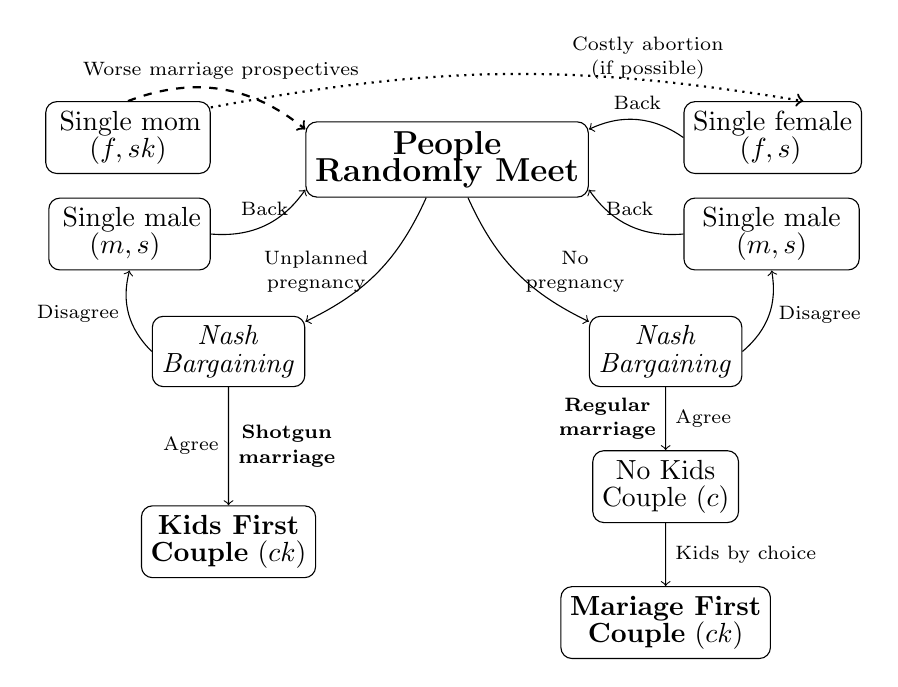
\begin{tikzpicture}[every text node part/.style={align=center}, scale=0.75]
   % Place nodes
   \node [block] (1) {\large \textbf{People}  \\[-0.5ex]  \large  \textbf{Randomly Meet}};
   \node [block, below left = 1.5 cm and 0.0 cm of 1] (2) {\textit{Nash} \\[-0.5ex] \textit{Bargaining}};   
   \node [block, below right = 1.5 cm and 0.0 cm of 1] (3) {\textit{Nash} \\[-0.5ex] \textit{Bargaining}};   
   \node [block, below = 1.5 cm of 2] (5) {\textbf{Kids First} \\[-0.5ex] \textbf{Couple} ($ck$)};
   \node [block, below = 0.8 cm of 3] (7) {No Kids \\[-0.5ex] Couple ($c$)};
   \node [block, below = 0.8 cm of 7] (8) {\textbf{Mariage First} \\[-0.5ex] \textbf{Couple} ($ck$)};
   \draw[->] (1) to [bend left = 20] node [left] {\scriptsize Unplanned \\[-0.75ex] \scriptsize pregnancy} (2);
   \draw[->] (1) to [bend right = 20] node [right] {\scriptsize No \\[-0.75ex] \scriptsize pregnancy} (3);
   \draw[->] (2) to node [left] {\scriptsize Agree} node [right] {\scriptsize \textbf{Shotgun} \\[-0.75ex]  \scriptsize \textbf{marriage}} (5);
   \draw[->] (3) to node [right] {\scriptsize Agree} node [left]  {\scriptsize \textbf{Regular} \\[-0.75ex]  \scriptsize \textbf{marriage}} (7);
   \draw[->] (7) to node [right] {\scriptsize Kids by choice} (8);   
    \node [block, above left   = 0.575 cm and -0.75 cm of 2] (4) {\,Single male \\[-0.5ex] ($m,s$)\,\,};
    \node [block, above left   = 1.8 cm and -0.75 cm of 2] (4-sm) {\,Single mom \\[-0.5ex]  ($f,sk$)};
    %\node [block, left = 0.2 cm of 4-sm] (4-nsm) {\,Single female \\[-0.5ex]  ($f,sk$)};
	\node [block, above right   = 0.575 cm and -0.75 cm of 3] (6) {\,\,Single male\,\,\\[-0.5ex] ($m,s$)};
    \node [block, above right   = 1.8 cm and -0.75 cm of 3] (6-f) {Single female\\[-0.5ex] ($f,s$)\,};   
    \draw[->] (2.180) to [bend left = 30] node [left] {\scriptsize Disagree} (4.270);
    \draw[->,thick,dotted] (4-sm.20) to [bend left = 10] node [above right=-0.2cm and 0.7cm] {\scriptsize Costly abortion \\[-0.75ex] \scriptsize (if possible)} (6-f.50);
    \draw[->] (3.0) to [bend right = 30] node [right] {\scriptsize Disagree} (6.270);
     \draw[->] (6.180) to [bend left = 30] node [above] {\scriptsize Back}  (1.-12);
   \draw[->] (6-f.180) to [bend right = 30] node [above] {\scriptsize Back} (1.12);
   \draw[->,thick,dashed] (4-sm.90) to [bend left = 30] node [above] {\scriptsize Worse marriage prospectives}  (1.168);
   \draw[->] (4.0) to [bend right = 30] node [above] {\scriptsize Back} (1.192);
   
\end{tikzpicture}
\caption{Transitions around the marriage market.\label{diagram}}
\end{center}
\end{figure}

\subsection{Couple and Child}
Let $V^{f,ck}_t$ and $V^{m,ck}_t$ represent the values of male and female of being in a couple with a child conditional on staying together in period $t$, and $V^{f,dk}_t$, $V^{m,dk}_t$ represent the value of divorce of such a couple. This section describes their recursive definition, starting from value $0$ in the last period.

The couple enters the period with savings $a$, bringing gross return $R\cdot a$, productivities $z^m$ and $z^f$, love shock $\psi$ and decision weights $\theta' = (\theta^f,\theta^m)$. Productivities, together with age, determine female and male wages $W^f_t(z^f)$, $W^m_t(z^m)$. The couple gets utility from spouses' consumption and the child's consumption; part of the latter can be produced at home by reducing the female labor supply. The love shock represents an additive utility surplus of being together.

Conditional on staying together in the period $t$, the choice of the couple are spouses' consumption $c^f$, $c^m$, expenditures on the child $x$, female labor supply $l^f$ and savings $a'$. I summarize the ``exogenous'' state by $\omega = (z^m,z^f,\psi)$. After making the decisions, the couple transitions to the next period $t+1$ and gets a draw of $\omega'$. Given $a'$ and $\omega'$ it chooses whether to divorce, which is represented by a binary indicator $d_{t+1}(a',\omega')$.  If it does not, it enters the next period with the decision weights $\theta'=\theta'(a',\omega',\theta)$, evolution of which is determined by renegotiation; otherwise the couple divorces.

The couple's decisions are defined by the following optimization problem and the continuation values:
\begin{align}(\tilde a',\tilde c^f,\tilde c^m,\tilde x,\tilde l^f)  = \argmax\limits_{a',c^f,c^m,x,l^f} \left\{\theta^f \cdot u(c^f) + \theta^m\cdot u(c^m) + \psi + \phi(q) + \beta\cdot \E_{\omega'|(l^f,\omega)} \mathcal{V}^{ck}_{t+1}\right\}
 \end{align}
\vspace{-2em}
\begin{align*}
\text{s.t. \ } & a' + c + x = R\cdot a  + W^m_t(z^f) + l_f \cdot W^f_t(z^m) & \text{(evolution of joint assets)},\\
                    & c =C(c^f,c^m) & \text{(increasing returns in consumption)},\\
                    & q = f(x,l^f) \geq \underline{q} & \text{(required costs of childcare)},
                  %  &  z^{f\prime} = z^f + \varepsilon^{z,f}_t - \delta(l^f) & \text{ (evolution of female productivity)}\\
				% &  z^{m\prime} = z^m + \varepsilon^{z,m}_t &  \text{ (evolution of male productivity)}\\
                   % & \psi' = \psi + \varepsilon^{\psi}_t & \text{(evolution of marriage surplus),}
\end{align*}
\vspace{-2em}
\begin{align*}
\text{where \ } & \mathcal{V}^{ck}_{t+1} =   (1-d_{t+1})\cdot \left[ \theta^f \cdot V^{f,ck}_{t+1}(a',\omega',\theta') +  \theta^m \cdot V^{m,ck}_{t+1}(a',\omega',\theta')\right]  & \text{(no divorce),} \\
& \hspace{2cm}+ d_{t+1}\cdot \left[ \theta^f \cdot V^{f,dk}_{t+1}(a',\omega',\theta') +  \theta^m \cdot V^{m,dk}_{t+1}(a',\omega',\theta')\right] & \text{(divorce).}
\end{align*}
Note that the decisions are homogeneous of degree $0$ with respect to $\theta$, which allows assuming $\theta^f + \theta^m = 1$. The corresponding individual continuation values are:
\begin{align}
V^{f,ck}_{t}(a,\omega,\theta)  = u(\tilde{c}^f) & + \psi + \phi(\tilde{q}) + \\\nonumber &\beta \cdot \E_{\omega'|(l^f,\omega)} \left\{ (1-d_{t+1}) \cdot V^{f,ck}_{t+1}(a',\omega',\theta')  + d_{t+1} \cdot V^{f,dk}_{t+1}(a',\omega',\theta') \right\},\\
V^{m,ck}_{t}(a,\omega,\theta)  = u(\tilde{c}^m) & + \psi + \phi(\tilde{q}) + \\\nonumber &\beta \cdot \E_{\omega'|(l^f,\omega)} \left\{ (1-d_{t+1}) \cdot  V^{m,ck}_{t+1}(a',\omega',\theta')  + d_{t+1} \cdot V^{m,dk}_{t+1}(a',\omega',\theta') \right\}.
\end{align}
The divorce decision and the law of motion for $\theta$ are defined in Section \ref{divorcedecision}. The divorce values $V^{\cdot,dk}$, and the child support assignment are given in Section \ref{divorcevalues}.

The transition for female productivity includes possible skill depreciation, which depends on the female labor supply's value $l^f$. Therefore the expectation operator is $\E_{\omega'|(l^f,\omega)}$. The transition laws are discussed in \ref{transition-laws}.

\subsection{Childless Couple}

Childless married couples have both partners working full-time. They enjoy the match quality stock $\psi$, and choose their consumption and savings. A childless couple may try to conceive a child. This decision precedes all consumption-savings decisions and happens after realizing the shocks and renegotiation, conditional on staying together at this period. The conception decision at the beginning of the following period is denoted by $k_{t+1}$. The decision problem is otherwise similar to those of a couple with a child:
\begin{align}(\tilde a',\tilde c^f,\tilde c^m,\tilde x,\tilde l^f)  = \argmax\limits_{a',c^f,c^m,x,l^f} \left\{\theta^f \cdot u(c^f) + \theta^m\cdot u(c^m) + \psi + \phi(q) + \beta\cdot \E_{\omega'|\omega} \mathcal{V}^{ck}_{t+1}\right\}
 \end{align}
\vspace{-2em}
\begin{align*}
\text{s.t. \ } & a' + c = R\cdot a  + W^m_t(z^f) + W^f_t(z^m) & \text{(evolution of joint assets)},\\
                    & c =C(c^f,c^m) & \text{(increasing returns in consumption)},
\end{align*}
\vspace{-2em}
\begin{align*}
\text{where \ } &   \mathcal{V}^{c}_{t+1} = \\
&  \hspace{-1cm} (1-d_{t+1})\cdot (1-k_{t+1})\cdot  \left[ \theta^f \cdot V^{f,c}_{t+1}(a',\omega',\theta') +  \theta^m \cdot V^{m,c}_{t+1}(a',\omega',\theta')\right]  & \text{(no divorce, no birth),} \\
&\hspace{-1cm} (1-d_{t+1})\cdot k_{t+1}\cdot  \left[ \theta^f \cdot V^{f,c\tilde{k}}_{t+1}(a',\omega',\theta') +  \theta^m \cdot V^{m,c\tilde{k}}_{t+1}(a',\omega',\theta')\right]  & \text{(no divorce, try birth),} \\
& + d_{t+1}\cdot  \left[ \theta^f \cdot V^{f,d}_{t+1}(a',\omega',\theta') +  \theta^m \cdot V^{m,d}_{t+1}(a',\omega',\theta')\right] & \text{(divorce).}
\end{align*}

I assume childbearing itself to be costless, but its success is random and uncertain. $p_t^{\text{success}}$ is assumed to be age-specific. Therefore, for a fertile couple, the value of trying to conceive a child is
\begin{equation}
V^{j,c\tilde{k}}_{t+1}(a',\omega',\theta') = p_t^{\text{success}}\cdot V^{j,ck}_{t+1}(a',\omega',\theta') + (1-p_t^{\text{success}})\cdot V^{j,c}_{t+1}(a',\omega',\theta'), \ \ j\in\{f,m\}
\end{equation}

The decision to conceive is based on a weighted value function \emph{after} the renegotiation (weighted with the next period's weights). Define the couple's weighted values as
\[V^{fm,c\tilde{k}}(a',\omega',\theta') = \theta^{f\prime} \cdot V^{f,c\tilde{k}}_{t+1}(a',\omega',\theta') + \theta^{m\prime} \cdot V^{m,c\tilde{k}}_{t+1}(a',\omega',\theta'),\]
\[V^{fm,c}(a',\omega',\theta') = \theta^{f\prime} \cdot V^{f,c}_{t+1}(a',\omega',\theta') + \theta^{m\prime} \cdot V^{m,c}_{t+1}(a',\omega',\theta'),\]
and the decision to (try to) give a birth is then
\begin{equation}k_{t+1}(a',\omega',\theta') = \I\left[ V^{fm,c\tilde{k}}(a',\omega',\theta')  \geq V^{fm,c}(a',\omega',\theta')\right].\end{equation}

There are two important remarks here. First, the value function $V^{fm,\cdot}$ is different from the weighted value function used in the couple's problem in the definition of $\mathcal{V}_{t+1}$ because of the timing of the decisions. This weighting is an artifact of the timing, and it makes decisions consistent with the broader limited commitment framework, dynamic complications of which are discussed in Marcet, Marimon, 2019. From a practice view, this formulation preserves homotheticity. However, it prevents writing the weighted terms as one value function, as they depend on a mixture of the current and expected future decision weights.\footnote{For a straightforward example, imagine that almost all bargaining weight belongs to the wife in a couple in the current period. Let $(\theta^f,\theta^m) = (1,\varepsilon)$ for some small $\varepsilon$. Suppose also that starting from the next period with certainty and forever $(\theta^f,\theta^m) = (\varepsilon,1)$. This situation has very low expected value for the wife, and it needs to be assessed accordingly, with decision weights reflecting the current state. Otherwise, the husband's future benefits are counted in the value function that now mostly reflects the utility of the wife.}



\subsection{Single Women and Men\label{singles-main}}

Each period single people may meet one potential partner with probability $p^{\text{meet}}$. The partners differ with assets and productivities $(a,z)$, and each match additionally receives a draw of initial marriage quality $\psi$, on top of this, with some chances men meet single mothers. The details of the partners market are described in \ref{marriagemarket}, right now we just denote the distribution of characteristics of the potential future matches by $\Gamma^M = \Gamma_{t+1}(a^M,z^M,\psi^M)$, and corresponding marriage decision $m^M = m_{t+1}(a^M,z^M,\psi^M)$ and resulting bargaining weight $\theta^M = \theta_{t+1}(a^M,z^M,\psi^M)$. So let $d\Gamma^M$ denotes the density of the matches with specified characteristics, and $\omega^M$ denotes future couple's exogenous state.

As I discuss above, there is a chance of $p^{\text{preg}}$ that an unplanned pregnancy happens when a potential couple meets. Given a match, the resulting marriage decision $m$ and the resulting bargaining weight $\theta$ may depend on pregnancy status, so I denote them $m^{m,p}$, $\theta^{m,p}$ when pregnancy happens and $m^{m,np}$, $\theta^{m,np}$ when it does not.

If unplanned pregnancy does not happen and woman agrees to marry, she enters a childless couple, that can later have a child and become a marriage-first couple. In unplanned pregnancy does happen and woman agrees, she enters a couple with a child, that is classified as a kids-first couple. 

In case of unplanned pregnancy both partners face social stigma $\phi_s$, that is expressed as a disutility of refusing to marry following an unplanned pregnancy.

Additionally, if woman refuses to marry she faces uncertain access to costly abortion: with a chance of $p^a$ she may choose to be a single mother or to abort the pregnancy with utility costs $\phi_a$, a chance of $1-p^a$ she stays a single mother. At the moment of marriage decision the realization of the abortion access is unknown.

Finally, the woman who refuse to enter the marriage following a pregnancy and kept the pregnancy may be awarded a child support. This happens with probability $p^{cs,n}$. Realization of the child support access happens after the pregnancy access and is uncertain at the moment of abortion decision, and the value of the child support is specific to the characteristics of the partner and the woman, as discussed in \ref{divorcevalues}. 

Therefore woman who rejects a proposal gets the following expected value:
\begin{equation}\label{sm-value}V^{f,sk?}_t(a,z^f) = p^{a}\cdot \max\left\{\E_{cs} V^{f,sk}(a,z^f), V^{f,s}_t(a,z^f) - \phi_a\right\} + (1-p^{a})\cdot V^{f,sk}_t(a,z^f).\end{equation}
where
\begin{equation} \E_{cs} V^{f,sk}(a,z^f) = p^{cs,n}\cdot V^{f,sk}_t(a,z^f+CS^m) + (1-p^{cs,n}) \cdot V^{f,sk}_t(a,z^f).
\end{equation}
The child support is match-specific, so this abuses the notation slightly.

Apart from the meeting of partners and pregnancies, the problem of the singles is a standard consumption-savings problem. Starting with single females:
\begin{align} & V_t^{f,s}(a,z^f)  = \max\limits_{a',c^f} \Bigg\{ \ \ u(c^f) +  \\\nonumber &  \beta\cdot \E_{z^{f\prime}|z^f} \Bigg( (1-p^{\text{meet}}_t)\cdot V^{f,s}(a',z^{f\prime}) \,+ & \text{(no partner met)}\\\nonumber
 & p^{\text{meet}}_t\cdot (1-p^{\text{preg}}_t) \cdot \int \Big[m^{M,np}\cdot V^{f,c}_{t+1}(a'+a^M,\omega^M,\theta^{M,np}) + & \text{(met, no pregnancy, agree)}\\\nonumber
 &\hspace{4cm}(1-m^{M,np})\cdot V^{f,s}_{t+1}(a',z^{f\prime}) \Big]d\Gamma^M + & \text{(disagree)} \\\nonumber
 & p^{\text{meet}}_t\cdot p^{\text{preg}}_t \cdot \int \Big[m^{M,p}\cdot V^{f,ck}_{t+1}(a'+a^M,\omega^M,\theta^{M,p})+  & \text{(met, shotgun marriage)}\\\nonumber
 &\hspace{2cm} (1-m^{M,p})\cdot \left\{V^{f,sk?}_{t+1}(a',z^{f\prime}) - \phi_s\right\} \Big]d\Gamma^M\Bigg) \Bigg\} & \text{(disagree, social stigma)}\\\nonumber
 \text{s.t. \ } & a' + c^f = R\cdot a  + W^f_t(z^f) & \text{(evolution of the assets)}.\\\nonumber
\end{align}

The single males face less consequences of unplanned pregnancies, as they do not have to make an abortion decision. Yet, they may be required to pay the child support and suffer from the same social stigma in case of refusal to enter a shotgun marriage. This depends on the female's match-specific decision to keep the pregnancy, so the value of refusal in this case:
\begin{equation}\label{man-cs}\E_{csm} V^{m,s}_{t}(a,z^{m}) = \begin{cases}p^{cs,n} \cdot V^{m,s}_{t}(a,z^{m}-CS^m)  + (1-p^{cs,n}) V^{m,s}_{t}(a,z^{m}), & \text{kept pregnancy}\\
  V^{m,s}_{t}(a,z^{m}), & \text{abortion}\end{cases}\end{equation}

Finally, the pool of potential partners for them is different, as there are chances they meet a single mother. In case this happens and they agree to marry, they face a one-time utility costs $\phi_r$, that is capturing disutility of having a step child. The decision problem for the males, defining $V^{m,s}_t(a,z^m)$ is described in the Appendix \ref{single-male-appendix}.


\subsection{Single Mothers}

Single mothers have sole custody of their children and pay the costs of them fully out of their labor income (that could have been adjusted in a past to account for the child support received). This can partially be done by a reduction in labor supply $l^f$.

They also have a chance to meet a single male, who has a utility loss $\phi_d$ from potentially having stepchildren, as shown in \ref{singlemaleproblem}. I refer to these losses as a remarriage penalty in the further parts.

The optimization problem and the value function definition therefore is
\begin{align} & V_t^{f,sk}(a,z^f)  = \max\limits_{a',c^f,x,l^f} \Bigg\{ \ \ u(c^f) + \phi(q) + \\\nonumber &  \beta\cdot \E_{z^{f\prime}|(l^f,z^f)} \Bigg( (1-p^{\text{meet}}_t)\cdot V^{f,s}(a',z^{f\prime}) \,+ & \text{(no partner met)}\\\nonumber
 & p^{\text{meet}}_t  \cdot \int \Big[m^{M,sm}\cdot V^{f,ck}_{t+1}(a'+a^M,\omega^M,\theta^{M,np}) + & \text{(met, agree)}\\\nonumber
 &\hspace{4cm}(1-m^{M,sm})\cdot V^{f,sk}_{t+1}(a',z^{f\prime}) \Big]d\Gamma^M\Bigg) \Bigg\}  & \text{(disagree)}\\\nonumber
 \text{s.t. \ } & a' + c^f + x = R\cdot a  + l_f\cdot W^f_t(z^f) & \text{(evolution of the assets)},\\\nonumber
                    & q = f(x,l^f) \geq \underline{q} & \text{(required costs of childcare)}.
\end{align}



\subsection{Shocks and Income Trends\label{transition-laws}}
I assume that shocks for productivity terms $z^f$, $z^m$ and love shock $\psi$ follow random walk process. For male productivity and love shocks the laws of motions are:
\begin{equation}\label{z-male-eq}
z^m_{t+1} = z^m_t + \varepsilon^{z,m}_{t+1}, \ \ \varepsilon^{z,m}_{t+1}\sim \mathcal{N}(0,\sigma^2_{z,m}),
\end{equation}
\begin{equation}\label{psi-eq}
\psi_{t+1} = \psi_t + \varepsilon^{\psi}_{t+1}, \ \ \varepsilon^{z,m}_{t+1}\sim \mathcal{N}(0,\sigma^2_{\psi}).
\end{equation}

The random walk structure with no mean reversion allows to interpret the productivity shocks as components of permanent income, therefore both female skills depreciation and the income reallocation through child support can be interpreted as shifts in $z$. The law of motion for the female productivity is
\begin{equation}\label{zoutlf}z^f_{t+1} = z^f_t + \varepsilon^{z,f}_{t+1} - \delta(l^f), \ \ \varepsilon^{z,f}_{t+1}\sim \mathcal{N}(0,\sigma^2_{z,f}), \ \ \delta(1) = 0.\end{equation}
The model assumes that women without children always have labor supply of 1, and women with children (both single and in couples) can reduce their labor supply as an input to the home production of the child's consumption $q$.

Finally, the labor earnings are determined by $z$ and age trends using the following expressions:
\begin{equation}\label{trends-eq}W^f_t(z^f) = \exp( \text{Trend}^f_t + z^f), \ \ W^m_t(z^m) = \exp( \text{Trend}^m_t + z^m).\end{equation}



\subsection{Marriage Market\label{marriagemarket}}
As all the decisions are homogeneous of degree 0 with respect to $(\theta^f,\theta^m)$, to lighten the notation since this part I assume that $\theta^f = \theta$ and $\theta^m = 1-\theta$, so in this part $\theta$ is a scalar. This also assumes that values of being in a couple, $V_t^{f,ck}$, $V_t^{m,ck}$ are monotonic with respect to $\theta$.\footnote{Numerical solutions may not exactly obey this monotonicity, but the modification of the conditions is straightforward. One important requirement to such a modification is that if, for example, female participation constraint binds, female bargaining power cannot decrease.}


Following Voena, 2015, I assume that men always meet women who are two years younger, and vice versa, which corresponds to the modal age difference in the US. The rest of the marriage market is as follows.

I assume that productivity of singles of each gender follows some exogenous (non-parametric) distribution over age, $F_t(z)$. Conditional on $z$, the distribution of log-assets is assumed to be truncated log-normal, namely, I assume that a latent variable is
\begin{equation}
\label{assets-partner}
\log a^*_t \sim \mathcal{N}(\mu^a_t(z),(\sigma^{a}_t(z))^2),
\end{equation}
and the realized actual value of assets is $a = a^*_t \cdot \I(a^*_t \geq \bar{a})$. This defines a distribution of available singles $F_t(z,a)$.\footnote{Regardless of characteristics, each individual draws potential partners from this distribution, so the mating is not assortative exogenously. Endogenously, however, people tend to agree more if the partner has similar characteristics, so there is endogenously generated assortativeness.}

After meeting a potential partner, the couple draws a realization of their match quality $\psi$ from a distribution $\mathcal{N}(\mu_{\psi,0},\sigma^2_{\psi,0})$.  The realization of this math quality is independent on the qualities of the partner. The match quality together with the potential partner's characteristics define distributions $\Gamma^M$ that are used in the definitions of the value function. 

For women, for instance, this is the distribution $\Gamma^f_t(a^m,z^m,\psi)$, that implies that, if they agree to marry, the couple will have $a = a^m + a^f$ and $\omega = (z^f,z^m,\psi)$. The agreement decision and the resulting bargaining weights are determined using the symmetric Nash Bargaining, there are three types of matches: regular match of childless singles without an unplanned pregnancy $(np)$, match with an unplanned pregnancy $(p)$ and males meeting single mothers $(sm)$. 

To lighten the notation, in this section we assume that the potential couple's characteristics $(a^f,a^m,z^f,z^m,\psi)$ are fixed, and therefore the value functions depend solely on $\theta$. The correct represetnation of the matching decision for the match type $q$ will be, however, $m_t^q(a^f,a^m,z^f,z^m,\psi)$, and I shorten this to just $m^q_t$.

\textbf{Case 1: regular match ($np$).} This is the case when two childless singles meet each other and no unplanned pregnancy happens. Upon agreement, the partners become a childless couple and receive the values $V_t^{f,c}(\theta)$ and $V_t^{m,c}(\theta)$. If disagree, they remain singles and receive $V_t^{f,s}$, $V_t^{m,s}$. Therefore the marriage decision is given by
\[m^{np}_t = \I(\Theta^{np}_t \neq \varnothing), \ \text{where} \ \Theta^{np}_t = \left\{ \theta \ : \ V_t^{f,c}(\theta) \geq V_t^{f,s}, \ V_t^{m,c}(\theta) \geq V_t^{m,s} \right\},\]
and the initial bargaining weight is defined as
\begin{equation}\label{bargaining-problem-regular}\theta^{np}_t = \argmax\limits_{\theta\in \Theta^{np}_t} \left[ V_t^{f,c}(\theta) - V_t^{f,s} \right] \times \left[ \vphantom{ V_t^{f,c}(\theta)}V_t^{m,c}(\theta) - V_t^{m,s} \right].\end{equation}

\textbf{Case 2: unplanned pregnancy ($p$).} This is the case when two childless singles meet each other and an unplanned pregnancy happens. There are hree important changes from the last case. First, both partners suffer social stigma $\phi_s$, altering their disagreement options. Second, women has a risk of becoming a single mother, and her expected value is described by \ref{sm-value}. Third, men pay child support and women receive child support, so men's value is also altered with $\E_{csm}$ operator as in \ref{man-cs}.\footnote{The timing of this bargaining is a little bit subtle. I assume that the woman cannot commit on whether to keep the pregnancy in case of the man's refusal to marry, and has to re-optimize the decision in this subgame.} The marriage decision is hence given by
\[m^{p}_t = \I(\Theta^{p}_t \neq \varnothing), \ \text{where} \ \Theta^{p}_t = \left\{ \theta \ : \ V_t^{f,ck}(\theta) \geq V_t^{f,sk?} - \phi_s, \ V_t^{m,ck}(\theta) \geq \E_{csm} V_t^{m,s} - \phi_s \right\},\]
and the initial bargaining weight is defined as
\begin{equation}\label{bargaining-problem-upp}\theta^{p}_t = \argmax\limits_{\theta\in \Theta^{p}_t} \left[ V_t^{f,ck}(\theta) - (V_t^{f,sk?} - \phi_s)  \right] \times \left[ \vphantom{ V_t^{f,ck}(\theta)}V_t^{m,ck}(\theta) - (\E_{csm} V_t^{m,s} - \phi_s) \right].\end{equation}

\textbf{Case 3: single mothers match ($sm$).} This is the case when single male meets a woman who already has a child from previous relationships. It is somewhat analogous to the previous case: if the couple agrees to marry, they become couple with a child (kids-first, for the record). However, a conceptual issue is that people generally do not like having stepchildren, and to compensate for this, I introduce a utility penalty to a potential husband $\phi_r$, which is paid as a one-time cost in case the male agrees to enter such a marriage. Additionally, as no new children are born, there is no child support assigned in this case. Therefore
\[m^{sm}_t = \I(\Theta^{sm}_t \neq \varnothing), \ \text{where} \ \Theta^{sm}_t = \left\{ \theta \ : \ V_t^{f,ck}(\theta) \geq V_t^{f,sk}, \ V_t^{m,ck}(\theta) - \phi_r \geq V_t^{m,s}   \right\},\]
and
\begin{equation}\theta^{sm}_t = \argmax\limits_{\theta\in \Theta^{sm}_t} \left[ V_t^{f,ck}(\theta) - V_t^{f,sk}  \right] \times \left[ \vphantom{ V_t^{f,ck}(\theta)} (V_t^{m,ck}(\theta) - \phi_r) - V_t^{m,s} \right].\end{equation}


\subsection{Renegotiation and Divorce Decisions\label{divorcedecision}}

The divorce decision happens before decisions on consumption, savings and labor supply, value of exogenous state $\omega = (z^f,z^m,\psi)$ is realized and couples has savings $a$ from the previous period.  At this moment individuals know their values of staying together and value of divorce. For couples with children, these are $V_t^{f,ck}$, $V_t^{m,ck}$ and $V_t^{f,dk}$ and $V_t^{m,dk}$ respectively. 

Given $a$ and $\omega$ I define two sets, that represent values of $\theta$ that are satisfactory for each partner:
\[\Theta^f_t(a,\omega) = \left\{\tilde \theta \ : \ V_t^{f,ck}(a,\omega,\tilde\theta) \geq V_t^{f,dk}(a,\omega)\right\},\]
\[\Theta^m_t(a,\omega) = \left\{\tilde \theta \ : \ V_t^{m,ck}(a,\omega,\tilde\theta) \geq V_t^{m,dk}(a,\omega)\right\}.\]
and their union:
\[\Theta(a,\omega) = \Theta^f_t(a,\omega) \cap \Theta^m_t(a,\omega).\]

The divorce therefore is defined:
\begin{equation}
d_t(a,\omega) = \begin{cases} 1, \ \ \Theta(a,\omega) = \varnothing,\\
 0, \ \ \Theta(a,\omega) \neq \varnothing.
 \end{cases}
\end{equation}

In case of $d_t = 0$, the evolution of $\theta$ is defined through this set. Namely, given $\theta$, and the next period's set $\Theta_{t+1}(a',\omega')$, if $\theta \in \Theta_{t+1}(a',\omega')$ the $\theta$ is kept at the same level, otherwise, it adjusts according to which participation constraint binds to ensure the lowest deviation.%, namely define $\theta^* = \argmin\limits_{t \in \Theta_{t+1}} |t - \theta|$. 

To be precise, for a non-empty set one can define $\theta^f_t(a,\omega) = \inf \Theta_t(a,\omega)$ to be the minimal bargaining power such that both participation constraints are satisfied. This corresponds to a point $\tilde{\theta}$ for which female participartion constraint exactly binds $V_t^{f,ck}(a,\omega,\tilde\theta) = V_t^{f,dk}(a,\omega)$ and $V_t^{m,ck}(a,\omega,\tilde\theta) \geq V_t^{m,dk}(a,\omega)$. In a symmetric manner I define $\theta^m_t(a,\omega) = \sup \Theta_t(a,\omega)$. Then, continuing to assume monotonicity,  
\[\theta \in \Theta_t \Leftrightarrow \theta^f_t \leq \theta \leq \theta^m_t,\]
and therefore the transitions for $\theta$ are defined through these two functions:
\begin{equation}\theta'(\theta,a',\omega') = \begin{cases} \theta, & \text{if \ }  \theta^{f\prime}(a',\omega') \leq \theta \leq \theta^{m\prime}(a',\omega'), \ \Theta'(a',\omega') \neq \varnothing,\\
\theta^{f\prime}, & \text{if \ }  \theta < \theta^{f\prime}(a',\omega'),\ \Theta'(a',\omega') \neq \varnothing,\\
\theta^{m\prime}, & \text{if \ }    \theta_t > \theta^{m'}(a',\omega'),\ \Theta'(a',\omega') \neq \varnothing,\\
\varnothing, & \text{if \ }  \Theta'(a',\omega') = \varnothing.
\end{cases}\end{equation}

This definition ensures the minimal deviation from the full commitment allocation, in which the bargaining weights are fixed. This maps into the classic limited commitment framework as in Marcet, Marimon, 2019: a Lagrange multiplier on a binding participation constraint corresponds to an increase in $\theta$ after rescaling, and the rescaling is possible because the decisions are homogeneous of degree zero in the bargaining weights.




%The divorce happens if there does not exists a pair of decision weights $\theta = (\theta^f,\theta^m)$ such that bo

\subsection{Divorce Values and Child Support\label{divorcevalues}}

When couple divorces, the assets are split evenly. This follows Voena, 2015, which provides a broader discussion of this assumption. Shortly, it is justified by the fact that most of the state either follow equal division of marital property or impose on average a division that is approximately equal, and the fact that people accumulate most of their wealth in marriage as they marry being relatively young. I did not find this to be particularly important for the qualitative results, although the property division obviously affects the divorce rates.

Instead, I assume that upon divorce both spouses incur fixed utility costs $\phi^d$. Therefore the divorce values are based on couple's state, and for the couples without children are given by 
\begin{equation}
V^{f,d}_t(a,\omega) = V^{f,s}_t(0.5\cdot a,z^f) - \phi_d, \ \ \ V^{m,d}_t(a,\omega) = V^{m,d}_t(0.5\cdot a,z^m) - \phi_d.
\end{equation}

If couple with a child divorces, the child custody is always given to mother, and the father does not get any utility from the absent child. The father, however, can be forced to pay child support. The permanent nature of productivity shocks $z$ allows to model child support as reallocation in productivities. The child support is assumed to be related solely to the male's labor income.

The child support is awarded following a divorce with probability $p^{cs,d}$, which is different between married and unmarried couples. If the child support is awarded, the evolution of productivity is $\tilde{z}^f_{t} = z^f_{t} + CS^m(z^m_t)$ and  $z^m_{t} = z^m_t - CS^f(z^f_t,z^m_t) $ for women and men respectively. Whether the child support is awarded is not known at the moment of divorce or marriage decisions. This realization does not keeps track of child's age, assuming the child support is paid indefinitely long, however, the fixed chances to avoid child support balance this. Productive males who lose the most because of indefinitely long payment period are also the most protected as they are less likely to pay relative to the case where establishing child support were up to decision of women.

To determine the exact change in $z$, assume that child support is proportion $\kappa$ of male's labor income, then the productivity loss for male $CS^m(z^m)$ sovles \[\exp(z^m_t  - CS^m +  T^m_t) = (1-\kappa)\cdot \exp(z^m_t  +  T^m_t),\] and the productivity gain of female $CS^f(z^f_t,z^m_t)$ solves \[\exp(z^f_t + CS^f +  T^f_t) = \exp(z^f_t  +  T^f_t) + \kappa \cdot \exp(z^m_t  +  T^m_t).\] 

Given the values for the child support, the (expected) values of the divorce for a couple with a child are
\begin{align}
V^{f,dk}_t(a,\omega) = p^a\cdot V^{f,sk}_t(0.5\cdot a,z^f + CS^f) + (1-p^a)\cdot V^{f,sk}_t(0.5\cdot a,z^f)  - \phi_d, \\
V^{m,dk}_t(a,\omega) = p^a\cdot V^{m,s}_t(0.5\cdot a,z^m - CS^m) +  (1-p^a)\cdot V^{m,s}_t(0.5\cdot a,z^m) - \phi_d.
\end{align}


In the actual solution the resulting transition of $z$ is approximated by two-point binary distribution over the nearest grid values. 




\subsection{Functional Forms}
The model assumes a set of standard CRRA utility and production functions.

Consumption's utility is standard:
\begin{equation}u(c) = \frac{c^{1-\sigma}}{1-\sigma}.\end{equation} When two spouses live in the couple, they can spend less money to achieve consumption levels $c^f$, $c^m$ then alone because of household's returns to scale. I assume that total couple's consumption expenditures are
\begin{equation}c = C(c^f,c^m) \equiv \left[ (c^f)^{1+\rho_c} + (c^m)^{1+\rho_c}\right]^{\frac1{1+\rho_c}}.\end{equation}

In a spirit of Chiappori, Mazzocco, 2017\nocite{chiappori2017static}, couple's intrahousehold problem can be simplified to picking just a total consumption expenditures. To see this, one may consider the problem
\[U(c) = \max_{c^f,c^m} \left\{ \theta^f\cdot \frac{(c^f)^{1-\sigma}}{1-\sigma} + \theta^m\cdot \frac{(c^m)^{1-\sigma}}{1-\sigma}, \ \ \text{ s.t. } \ \ c = \left[ (c^f)^{1+\rho_c} + (c^m)^{1+\rho_c}\right]^{\frac1{1+\rho_c}}\right\}.\]
After doing some algebra, it can be shown that there are functions $A(\theta)$, $k_f(\theta)$ and $k_m(\theta)$ such that
\begin{equation*}U(c) = A(\theta)\cdot \frac{c^{1-\sigma}}{1-\sigma}, \ \ c^f = k^f(\theta)\cdot c, \ \ c^m = k^m(\theta)\cdot c,\end{equation*}
and therefore utility of the couple can simply be represented as a function of total expenditures and bargaining weights, which simplifies the optimization considerably.

When the children are present, parents produce child's consumption $q$ as a public good. Both parent's money $x$ and female time $l^f$ contribute to the its production, so \begin{equation}q = f(x,l^f) \equiv \left[ x^{\lambda} + \kappa\cdot (1-l^f)^{\lambda}\right]^{\frac1\lambda}\end{equation} This function is built in such a way that if female works full-time ($l^f = 1$), $q$ just represents the monetary expenditures $x$. This also helps to interpret the subsistence constraint, as we require $q \geq \bar{q}$.

The utility of having a child consists of fixed utility benefit and part that is dependent on the child's consumption, so
\begin{equation}\label{child-q}\phi(q) = \phi_0 + \alpha\cdot \frac{q^{1-\phi_1}}{1-\phi_1}.\end{equation}

For the skills depreciation functions, the model assumes discrete choice of labor supply, which only has an extensive margin: whether or not to participate in the labor market. Participating corresponds to $l^f = 1$ and $\delta(1) = 0$, and non-participating is $l^f = \underline{l}$ and $\delta(1) = \underline{\delta}$. 




\subsection{Additional Details}
All agents retire at the age of $T^R$, where they get a fixed retirement income of $b$, unconditional on their past productivity. I found this to be of minor importance for the results, as all the transitions I focus only happen early in life.

By computational reasons, the value of love shock actually received by couple is clipped to fit to be within $[\underline{\psi},\overline{\psi}]$, which are set to be 2.5 of \emph{initial} standard deviation. This can be intepreted utility contribution of $\psi$ being $u^{\psi} = \min\{\max\{ \underline{\psi}, \psi \},\overline{\psi}\}$. As standard deviation is large and $\psi$ is assumed to be a random walk, this prevents gains from marriage to increase indefinitely over the lifetime without altering the stochastic process. This way agents with two very high $\psi$ are still different: the one with the larger value has smaller probability to fall below a certain number.

I introduce non-linear taxation, that depends on couple's or single's total labor earnings and number of children, following the approximations obtained by Guner et al, 2012\nocite{guner2012taxation}. The approximations are based on social security data and capture not solely the tax schedule, but also the average utilization of the major welfare programs, including EITC and TANF.

\section{Quantification Approach}

The model has a great degree of flexibility, which is achieved by a large number of parameters. Some of them can be estimated outside the model and fixed externally, however, there is a number of crucial preference and transition parameters that cannot be inferred directly as they affect many outcomes simultaneously, for them an estimation procedure is needed.

To solve the model, all state variables and transition probabilities are discretized, and the value function iteration starting from the very last period is used. An important complication is that there is no guarantee that value functions are convex or even monotonic, although the latter can be proved in simple cases. The discreteness of marriage, divorce, fertility and labor supply decisions and the collective nature of the couple's decisions make modern Euler-equation based methods (like Iskhakov et al, 2015\nocite{iskhakov2015estimating}) difficult to apply. Adding taste shocks as a smoothing device can potentially be done, but it is not enough to obtain tractable Euler equations as the envelope theorem is not applicable to the individual values of couple's decisions. Therefore the preferred approach is maximal discretization, and the consumption-savings problems are solved by brute force global search. The details of the method are described in Appendix \ref{solution-appendix}. 

In total, the model takes around three minutes to be solved and simulated on a Macbook Pro, 2015. As the routines for optimization, marriage and renegotiation are very parallelizable, it can be efficiently solved on GPUs. Running time is then 30--70 seconds, depending on the GPU model.

\subsection{Strategy}
To provide more focused evidence and also to facilitate understanding the education differences in the shotgun marriage patterns, I perform estimation on two distinct subsamples: college graduates and high school graduates. As Table \ref{share_table_0} suggests, the college graduates have substantially larger differences between kids-first and marriage-first couples in terms of divorce, and this difference is mostly expressed in the lower divorce rates for the marriage-first group. This makes comparing two separate instances of the estimated model particularly promising.

This approach is similar to Low et al, 2018, who study welfare utilization and consider only the lower-education subsample. Similar to them, yet slightly unrealistically I assume that college graduates always marry college graduates and high school graduates always marry high school graduates.

I mainly use ACS data as my key empirical results are obtained from there, however, for the purpose of external estimation of things that are not observed in ACS I utilitze SIPP data. Finally, few estimation targets are taken from literature. 

\subsection{Ex-Ante Fixed Parameters}
The agents being at age 21 for females (23 for males), retire at 65 (67) with $0.4$ of median income as a pension benefits (on top of their savings) and die deterministically at 75 (77), leaving no bequest.

Following the standards in the lifecycle literature I take $\beta = 0.96$ and $R = 1/\beta$ (see ... for references).

For the labor supply side, the drift $\delta(\underline{l})$ is set to $0.09$ for college graduates and $0.06$ for high school graduates, so woman loses roughly 9\% or 6\% of her income per 1 year out of labor force. These numbers replicate structural estimates of Adda, Dustmann, Stevens, 2017\nocite{adda2017}, despite them being on German Data. Blasutto, 2020 gets similar numbers through structural estimation of a model similar to this on PSID. Additionally, those out of labor force are assumed to have $\underline{l} = 0.2$ instead of zero, so they still get one-fifth of their regular income. This assumption is mostly for computational reasons, but also reflects heterogeneous potential for home production.

For the preference side, I assume intertemporal elasticity of substitution in consumption to be a standard number $\sigma = 1.5$, and I assume that this elasticity is the same for the child's consumption (equation \ref{child-q}), so $\phi_1 = \sigma = 1.5$. For the returns to scale within a couple I fix $\rho_c = 0.23$ following Voena, 2015, which indicated mildly increasing returns to scale. In the child's quality production function $f(x,l^f)$ the substitutability between money and time is assumed to be high and is set to be $\lambda = 0.7$, as in Sommer, 2015.

For the child support enforcement, I assume that the value of the child support assigned corresponds to 20\% of male's income, that is considered to be an modal value in the US (see ...). For the enforcement strengths, I assume that $p^{a,{nm}} = 0.284$ of never married women and $p^{a,{nm}} = 0.461$ of divorced women get child support, these numbers correspond to the statistical share of eligible mothers receiving the child support in 20??, see ....

For the success in a child's conception I use the following success probabilities: 86\% at 21--24, 78\% at 25--29, 63\% at 30--34 and 52\% at 35--40 (see Rosental, 2002\nocite{rosenthal2002fertility}). These numbers reflect chances of women to get pregnant within a year if using no birth control. More modern Kennes, Knowles, 2012\nocite{kennes2012} use somewhat higher chances, but they model infertility and have taste shocks that may prevernt childbearing, so I pick the lower values to balance this. I assume that infertility is deterministic at starts at 41.

At the beginning of the life $2\%$ of college graduate women and $20\%$ of high-school graduate women have kids. I assume that by the age of 21 nobody is married, which is counterfactual, but does not determine the results. Everyone starts with zero assets, initial distributions of productivities are based on the data, as described below. 

The scale of all income-like numbers is thousands of $2017$ USD. I restrict assets choices such that no one can have more that $\$ 1m$ in savings, this constraint is binding for a small share of individuals. 

\subsection{Externally Estimated Parameters}

Three crucial objects to estimate from the data are the variance of income shocks, the distribution of assets and productivities singles and the income trends. The variances require observing individual over time and the distribution requires the assets data, none of which is possible using the ACS data. Therefore for them I use SIPP data, 2014 Waves 1--3, that cover three years. To be more in line with the main data, the income trends are still estimated using the ACS, as SIPP estimates are less smooth, and the described SIPP technique does not utilize dynamic structure in estimation of the trends.

\subsubsection{SIPP: Income Shocks and Distribution of Singles}
For SIPP, I impose the following restrictions on the data, replicating the approach that is done in Section \ref{empirical-section} for ACS. I treat as working those who work at least 10 hours per week. I drop people with hourly income less than one-half of the federal minimum wage and with hourly income above $95\%$ quantile of the distribution, I also drop those whose income went up or down more than four times in two consecutive years.

The estimation approach follows Meghir, Pistaferi, 2004\nocite{meghir2004income}. Endogenous choice of female labor supply is an important concern in estimating the individual productivity shocks, therefore a Heckman correction is used.

At the first stage the labor force participation regression is estimated, using presence of the mortgage as an excluded instrument (following Blundell et al, 2016\nocite{blundell2016consumption}, it is supposed to increase labor force participation regardless of productivity). At the second stage, the log wage is regressed to this Heckman correction, together with a set of dummy variables for age, state and year, and the residuals (corrected) are used to obtain the values of productivity $z$ for those in labor force. At the third stage, based on these residuals a simple GMM time-series procedure is used to split the variation in these residuals onto the permanent income components and measurement error. The details of the estimation are given in Appendix .... 

Then, I use the same residuals to estimate distribution of singles. It is done in two steps. First, I estimate the distribution of $z$ non-parametrically: given the grid values at each age and $z$ that are observed in the data I can assign weights according to proportion of singles with $z$ that are closest to a certain grid point. This gives me probabilities of each productivity grid point at each age.

Then, I estimate a heteroskedastic Tobit regression of log-assets conditional on $z$, treated people with assets less than $\bar{a}$, that includes zero, as censored observations. I prefer parametric approach as assets data are noisy, and treating them non-parametrically produces undesirable patterns.  The regression specification is
\begin{equation}\label{tobit-partner}
\log a_t^* = \alpha_0 + \alpha_1\cdot t + \alpha_2 \cdot z + \alpha_3 \cdot z\cdot t + \sigma_t \cdot \varepsilon_t, \ \ \sigma_t = e^{\beta_0 + \beta_1\cdot t}, \ \ a_t = a_t^* \cdot \I(\log a_t^* \geq \bar{a}),
\end{equation}
and I take $\bar{a} = 0$ in the estimation.\footnote{Income and assets are measured in thousands of dollars, so this treats all people with net worth below \$1000 as having zero assets.} The model is estimated via standard MLE.

For males, the standard errors of productivity shocks and the distribution of singles are estimated similarly, but without the Heckman correction. For the distribution of singles, women with and without kids were split, and the share of single mothers was estimated non-parametrically (as just percentages in the data). 

As SIPP data are monthly, yearly per-hour earnings were assembled out of monthly earnings and hours, and average net worth during a year was used for assets.

\subsubsection{ACS: Income Trends}
The income trends are estimated on ACS separately, where the data is treated in the same way as in Section \ref{empirical-section}. To get rid of the intensive margin of labor supply, the per-hour earnings are converted to yearly assuming that everyone works 2080 hours per year.

The trend is assumed to be non-parametric. The earnings are regressed on a set of dummy variables for each age, 21--50 for females and 23--50 for males, past this point it is assumed to be flat. The regression additionally controls for race, state, survey year and metropolitan area status. I ignore the female labor force participation margin. Theoretically, ignoring this selection causes my estimated to overestimate the real trend, on the other hand, as there is skills depreciation from being out of labor force, the agents in simulated model will be on average below the trend, and I view these two factors as compensating each other. Appendix ... provides the regression specification.

\subsection{Internally Estimated Parameters}
Things to be estimated in the model are:
\begin{enumerate}
\item Preference parameters: additive utility from having a child $\phi_0$, weight of child's consumption in utility $\alpha$, productivity of female labor at home $\kappa$, subsistence constraint for the child's consumption $\bar{q}$
\item Characteristics of unobserved match quality $\psi$: initial distribution parameters $\mu_{\psi,0}$ and $\sigma_{\psi,0}$, the variance of match quality shocks $\sigma_{\psi}$.
\item Reduced-form preference shifters: disutility of divorce $\phi_d$, disutility of marrying a single mother for male $\phi_r$, disutility of not entering a shotgun marriage (social stigma) $\phi_s$.
\item Abortion access and costs: probability to get abortion access $p^{a}$ and utility costs of abortion $\phi_a$.
\item Probabilities to meet a partner $p^{\text{meet}}_t$ and to have an unplanned pregnancy $p^{\text{preg}}_t$.  I parametrize them with values at three age points: $(p^{\text{meet}}_{21},p^{\text{meet}}_{30},p^{\text{meet}}_{40})$ and $(p^{\text{preg}}_{21},p^{\text{preg}}_{28},p^{\text{preg}}_{35})$ and interpolate with quadratic function in between these points.
\end{enumerate}

In total this gives 12 choice parameters and 6 transition probabilities. I define the resulting parameter vector to be
\begin{equation}\label{theta-eq}
\Theta = \left[ \phi_0,\alpha,\kappa,\bar{q},\mu_{\psi,0},\sigma_{\psi,0},\phi_d,\phi_r,\phi_s,p^{a},\phi_a,p^{\text{meet}}_{21},p^{\text{meet}}_{30},p^{\text{meet}}_{40},p^{\text{preg}}_{21},p^{\text{preg}}_{28},p^{\text{preg}}_{35}\right],
\end{equation}
which is 18-dimensional. 

To discipline these parameters, I use overidentifying set of moment restrictions derived from the ACS. They include timings of divorce and fertility over duration of marriage, and percentage married, divorced and single with and without kids by age, with few other auxiliary things for pinning down preferences.

I use three external targets that are not available in ACS: share of child-related expenditures in labor earnings from Lino, 2001\nocite{lino2001expenditures}, percentage of unplanned pregnancies aborted from [...] and ratio of number of abortions at 30s over number of abortions at 20s from [...].

To tie the numbers together, I also introduced additional overidentifying restriction imposing certain marital sorting. For married women at 30 with income above median I compute what percentage of their husbands have income above median. In the model this is computed as $\P(z^m>0|z^f>0)$ among married couples. I refer to this as an income sorting measure.

Table \ref{targets-table} describes all the targets used and gives a rough idea of identification directions.  The total number of targets used is 95. The following section describes identification in more details.

\begin{table}[h]
\begin{center}
\caption{\label{targets-table}Estimation targets and parameters related to them.}
{\small
\begin{tabular}{p{0.5\linewidth} p{0.4\linewidth}}
\textbf{Target} &\textbf{Informative about} \\\hline
\% divorced $x$ years after marriage if kids-first, \ \ \ \ \ \ \% divorced $x$ years after marriage if marriage-first, $x \in \{1,...,10\}$ & Match quality shocks $\sigma_\psi$, divorce costs $\phi_d$, social stigma $\phi_s$  \\\hline
\% of kids-first and \% of marriage-first in female population at age $a$; \% of kids-first in population of married once \& with kids at age $a$; $a \in \{23,...,35\}$ & Unplanned pregnancy probabilities $p^{\text{preg}}_t$, meeting probabilities $p^{\text{meet}}_t$, fertility parameters $(\alpha,\phi_0,\bar q)$\\\hline
\% never married  without kids at age $a$, $a \in \{23,...,35\}$ & Meeting probabilities $p^{\text{meet}}_t$, match quality initial distribution $(\mu_{\psi,0},\sigma_{\psi,0})$ \\\hline
\% never married with kids at age $a$, \% divorced with kids at age $a$, \% divorced without kids at age $a$, $a \in \{28,...,35\}$ & Meeting probabilities, match quality initial distribution $(\mu_{\psi,0},\sigma_{\psi,0})$, match quality shocks $\sigma_\psi$, step children penalty $\phi_r$ \\\hline
\% of women with more than one marriage at 40 & Meeting probabilities $p^{\text{meet}}_t$, step children penalty $\phi_r$ \\\hline
\% of couples with kids $x$ years after marriage, $x \in \{4,...,8\}$ (if still married) & Fertility parameters $(\alpha,\phi_0,\bar{q})$ \\\hline
\% in labor force if with kids and married at 30 & Labor productivity at home $\kappa$ \\\hline
\% of child expenditures in total earnings${}^*$ & Fertility parameters $(\alpha,q)$ \\\hline
\% unplanned pregnancies aborted${}^*$, ratio of abortions at 30s to abortions at 20s${}^*$ & Abortion access and costs $(p^a,\phi_a)$\\\hline
\% husbands with income above median for women with income above median (marital sorting) & Extra identification for match quality distribution $(\sigma_\psi,\sigma_{\psi,0},\mu_{\psi,0})$ \\\hline\hline
\multicolumn{2}{p{0.9\linewidth}}{\emph{Notes:} ${}^*$ denotes external targets, the sources are described in text. All other targets are computed on ACS following the methodology of Section \ref{empirical-section}.}\\
\hline
\end{tabular}
}
\end{center}
\end{table}

\subsection{Identification}
Each parameter affects multiple targets simultaneously, and this is the reason a proper estimation procedure as opposed to simple calibration is used. Nevertheless, for each parameter there is an idea about what set of targets is the most informative about it.

Meeting probabilities $p^{\text{meet}}$ are disciplined by share of never-married people over age and the share of kids-first and marriage-first couples. Unplanned pregnancy probabilities $p^{\text{preg}}_t$ are pinned down with share of kids-first couples, especially relative, share of never married women with kids and, less importantly, by percentage of abortions.

The size of match quality shock $\sigma_{\psi}$ is identified by steepness of divorce profile by marriage duration, looking especially at the marriage first group as the least vulnerable to divorce. The overall size of the divorce rates is informative about divorce cots $\phi_d$, and the difference between kids-first and marriage-first is easily affected by the size of social stigma $\phi_s$, among other factors that I discuss later.

The initial distribution of match quality is determined by percentage of never married people over age with and without kids. The latter group is particularly important as single in the model they certainly met at least one partner. Together with the share of women with more than one marriage at 40 these numbers are also informative about the meeting probabilities. The income sorting measure provides additional information, as it essentially picks the importance of income relative to the match quality in the partner selection process.

Steepness of age profile of fertility, represented by share of the marriage-first people in general population, is informative about the role of child's consumption in utility, $\alpha$. It is also affected by the expenditure share of couples, but the latter is determined more directly with the subsistence constraint parameter $\bar{q}$, although the separate identification of two parameters is a little subtle. The constraint $\bar{q}$ is also affected by the share of kids-first couples, as it is the most direct factor making raising children alone undesirable.
 
Overall level of fertility from the share of marriage-first couples and percentage of couples with kids by years after marriage are informative about overall benefits from having kids $\phi_0$. Additionally, the size of $\phi_0$ versus the scale of love shock is identified by comparing the share of divorced people with and without kids.

Productivity of female labor at home $\kappa$ is almost solely determined by the level of female labor supply. Similarly, the share of unplanned pregnancies aborted determines abortion access $p^a$, and the age profile of abortions is informative about their utility costs $\phi_a$.

Utility loss for having stepchildren $\phi_r$ is determined by percentage of divorced and never married women with kids, especially relative to those without kids, as the dynamics of their relative proportion is informative about changes in the remarriage chances.

\subsection{Simulated Method of Moments}

For every combination of parameters $\Theta$, I solve the model, obtain decision rules, simulate a sample of agents and track their decisions. Based on these decisions, I get simulated data, from which I compute the targets, replicating the way they computed in the data as close as possible. Based on the targets in the data and in the model, I compute the weighted GMM-style distance, and this number represents the overall fit of the model. I use optimization routine to select parameters $\Theta$ maximizing the overall fit of the model, i.e. minimizing this distance.

Formally, let the vector of the data targets be $t$ and the simulated values of the stargets from the model be $m(\Theta)$. The simulated method of moments distance function is a scalar
\[d(\Theta) = \left[ m(\Theta) - t\right]' \cdot W \cdot  \left[ m(\Theta) - t\right].\]

The weighting matrix corresponds to standard errors of the targets in the data, inverse and squared. In a canonical GMM framework the correlation of the targets should also be computed, however, following ... I ignore the covariances and assume the matrix is diagonal, prioritizing finite sample properties of the estimates over theoretical statistical efficiency.

I use standard errors obtained from ACS, except for external moments (marked with stars in Table ...). For the external moments I arbitrarily set standard error of $0.001$, which corresponds to standard error of the ACS numbers of similar magnitude. Finally, as this is central in my model, I artificially multiply the standard errors of shares of people divorced by the years after marriage in KF and MF groups by 1/4 to prioritize fitting these targets. 

The model simulates lifecycle of $15{,}000$ women. I did not find random sampling important for the targets I use as most of them are conditional on age or particular marriage duration, so for the sake of faster computations I treat women in each period as separate independent observations. To mitigate the concerns, I compute the moments three times with different sequences of the random draws and average among them.

For the optimization procedure I follow Arnoud et al, 2019\nocite{arnoud2019benchmarking}. There are many discrete decisions and there is noise coming from simulations, that makes the distance function $d(\Theta)$ non-smooth, although most of the approximated underlying decisions are expected to respond smoothly on changes in parameters. 

Therefore a two-step optimization procedure TikTak is used: it first performs global search and then runs many local optimizers. First, I take $20{,}000$ candidate values for $\Theta$ from quasi-random Sobol sequence for potential parameters values (rescaled to fit some reasonably wide bounds). Among them, I pick $250$ points with the lowest value of the distance to a sequence $\{\Theta^{1i}\}_{i=1}^{250}$.

Then I run sequence of local optimization procedures. At the first stage I take the best of these 250 points as a starting point. At the stage $i = \{2,...,250\}$, the starting point is a weighted average of the best point found at stage $i-1$ and the $\Theta^{1i}$, where the weight of the best point is growing with $i$.\footnote{I use $w_b = \max\{0.1,\min\{(i/250)^{0.5}\},0.995\}$ following the original paper.}

For the local optimizers, I use non-gradient regression-based nonlinear least squares algorithm DFO-LS, that is developed in Cartis et al, 2019\nocite{dfols}. Other potential choice is Nelder--Mead, the gradient-based methods are found to be extremly inefficient because of the stochastic noise in the function.

This algorithm is easily parallelizable, if in the weighted average instead of picking the point from stage $i-1$ the optimizer just uses the best point found so far. As the time it takes to evaluate the function at one point on GPU is approximately 1 minute, running running 15--20 concurrent optimization routines simultaneously (with each evaluating function 120--180 times) delivers reasonably stable and replicable results within less than 24 hours.

\iffalse
\subsection{Non-Parametric Probability Refinement}
In the main estimation exercise I parametrize probabilities of meeting and pregnancy by two second degree polynomials. As an additional step, after using the method describe above and obtaining a solution with a satisfactory fit, I implement the following estimation procedure aimed to mitigate the effects of this assumption. The parameter vector $\Theta$, defined in \ref{theta-eq}, can be split onto
\[\Theta = [ \Gamma, P],\]
where $P$ are the pregnancy and meeting probabilities and $\Gamma$ are choice parameters. Initial estimates from the TikTak algorithm imply $\Theta_0 = [\Gamma_0,P_0]$, where $P_0$ are given by the values of the quadratic.

Given the fixed decision rules $d(\Gamma_0,P_0)$ during the model simulations I can pick sequence of new transition probabilities $P_1$ that match share of single agents and share of kids-first couples by age exactly. Then the point $\Theta_{01} = [\Gamma_0,P_1]$ is used a starting point for a new estimation of decision parameters $\Gamma$, that allows to get $\Theta_1 = [\Gamma_1,P_1]$. Given $\Theta_1$, new probabilities $P_2$ matching the data can be found, $\Theta_{12}   = [\Gamma_1,P_2]$ used as a new starting point, and the process repeats. When the difference in probabilities $|P_{n} - P_{n-1}|$ is small enough, the estimates converge. The convergence is not guaranteed, but is achieved pretty quickly in the actual problems. 

To get the intuition about how data identify the meeting probabilities, imagine the following simplistic examples. Suppose the decision rules are such that one-half of all partners are accepted, and suppose $100\%$ of population are single at $22$ and $80\%$ of population are single at $23$. Then, $20\%$ of singles transition to non-singles, and this implies that $40\%$ of people meet potential partners.

Similar logic applies to the unplanned pregnancy probabilities. If $20\%$ of pregnancies end in shotgun marriages, and number of people having shotgun marriage goes from $0$ at $22$ to $1\%$ at $23$, then $5\%$ of people got unplanned pregnancies, so $p^{\text{meet}}_{22}\cdot p^{\text{preg}}_{22} = 0.05$. If $p^{\text{meet}} = 0.4$ as above, this implies $p^{\text{preg}} = 0.125$.

In the real model, the acceptance probabilities are heterogeneous and depend on the current distribution of characteristics, additionally, the value of $p^{\text{preg}}$ affects the acceptance probabilities for the general population. However, running a simple optimization procedure targeting new shares of singles and kids-first couples allows to get the values matching them exactly fairly quickly. Due to the distribution at each stage being random, there is some randomness in the probability estimates too, but running them several times and averaging provides an adequate result.

Past 35 years, where most of the transitions are over and share of singles is small, the estimation technique just assumes the fixed meeting and pregnancy probabilities at the average level of 33--35. 

\fi

\section{Estimates and Fit}

In this section I present the estimates in the model on two subsamples: high school graduates and college graduates. For the purpose of further comparison, I prioritize the fit for the college graduates, as they have more evident patterns related to the shotgun marriages. I estimate the full set of the model parameters on a subsample of college graduates. Then I fix the preference parameters $\bar{\Theta} = (\sigma_{\psi},\sigma_{\psi,0},\mu_{\psi.0},\phi_0,\alpha,\kappa)$ at the level of these estimates, and re-estimate the remaining set of parameters on the data for high school. As the preference parameters directly drive fertility timing by marriage duration, share of child-related expenditures and the labor force participation, I do not use these targets in the high school estimation.

Table \ref{par-estimates} presents parameter estimates for low and high-education samples. Table \ref{model-fit-table} presents the model fit and references the fit graphs representing the model fit.  Additionally, Table \ref{ext-estimates} presents external parameter estimates for income process and distribution of singles. 

The fit for the college graduates is exceptionally good, especially given the large number of targets. There only important issue is fertility timing: due to the absence of taste shocks, many couples are close to indifference between when to have children, and in particular, a number of couples, especially elder ones close to the fertility limits, try to conceive quickly after they are married. This is an artifact of the model rather than desirable property. Uncertain conception probability mitigates this slightly, but the most obvious solution is just to remove the first three years after marriage from the targets, which I did.

Since the high school model is estimated on restricted parameter set, it has generally worse fit, but still matches the main targets of the divorce rates of kids-first and marriage-first couples very decently. The share of kids-first and marriage-first couples, on the other hand, has significant discrepancy, though the overall pattern is similar. I see two reasons for this. First, a significant share of singles marry and have children earlier in life, and in the model the earliest moment married couple can have children is 22. The estimator solves this by inflating the meeting probabilities in early life, but this creates an undesirable pattern ($u$-shaped parabola) for the rest of the life. %This is possible to solve with more flexible parametrization, but this is not the main focus of mine yet. 

\def\f#1{\multicolumn{2}{l}{\hspace{0.75cm}Figure #1}}
\begin{table}[h]
\begin{center}
\caption{Model Fit\label{model-fit-table}}
\begin{tabular}{l r r r r}\hline\hline
& \multicolumn{2}{c}{\textbf{College}} & \multicolumn{2}{c}{\textbf{High School}} \\\hline
& \textbf{Model} & \textbf{Data} & \textbf{Model} & \textbf{Data} \\\hline
{\footnotesize {\% divorced 1--10 years after marriage if KF and MF} } & \f{\ref{fit-col-1}} &  \f{\ref{fit-hs-1}} \\
{\footnotesize {\% KF and MF at 23--35, in population and relative} }& \f{\ref{fit-col-1}} &  \f{\ref{fit-hs-1}} \\
{\footnotesize \% with kids 4--8 years after marriage } & \f{\ref{fit-col-1}} &  \f{\ref{fit-hs-1}${}^*$}\\\hline
{\footnotesize \% divorced with and without kids at 28--35 } & \f{\ref{fit-col-2}} &  \f{\ref{fit-hs-2}}\\
{\footnotesize \% never married with kids at 28--35 } & \f{\ref{fit-col-2}} &  \f{\ref{fit-hs-2}}\\
{\footnotesize \% never married without kids at 23--35 } & \f{\ref{fit-col-2}} &  \f{\ref{fit-hs-2}}\\\hline
{\footnotesize  \% with more than one marriage at 40} & 6.8 & 11.9 & 9.6 & 17.1 \\
{\footnotesize \% in labor force at 30 if married and kids} & 74.2 & 74.0 & 53.6 & 54.7${}^*$ \\
{\footnotesize mean \% of child expenditures in total earnings} & 40.6 & 40.0 & 39.3 & 40.0${}^*$ \\
{\footnotesize \% unplanned pregnancies aborted} & 39.9 & 40.0 & 37.3 & 40.0 \\
{\footnotesize abortions in 30s as \% of abortions in 20s} & 38.5 & 38.5 & 39.5 & 38.5 \\
{\footnotesize \% husbands above median if wife above median} & ... & ... & ... & ...\\
\hline
\multicolumn{5}{p{0.85\linewidth}}{\footnotesize \textbf{Notes:} KF refers to the kids-first women, MF refers to the marriage-first women. 23--35 refers to all ages from 23 to 35 and so on. ${}^*$ shows the numbers not targeted in the high school calibration.}\\\hline\hline
\end{tabular}

\end{center}
\end{table}



%One important issue for the high school group is that many people with lower education marry and have kids early, but the lifecycle in the model starts at 21. This can be seen by very high assigned probabilities in early life. Overcoming these issues is not hard, but introducing differences in the time bounds makes comparisons subtle.

%Appednix ... presents the unrestricted estimation, which has slightly better but also potentially less comparable results.


\begin{table}
\begin{center}
{\small
\caption{Estimated parameters.\label{par-estimates}}
\begin{tabular}{l p{0.35\linewidth} l l}\hline
\textbf{Parameters}  & \textbf{Description} &  \textbf{College} & \textbf{High School (R)}  \\\hline
$(\phi_0,\alpha)$ & Fertility preferences & $(0.30,0.45)$ & $(0.30^*,0.45^*)$ \\
$q$ & Required childcare costs & $34.39$ & $1.23$ \\
$\sigma_\psi$ & Match quality shock size & $0.67$ & $0.67^*$ \\
$(\mu_{\psi,0},\sigma_{\psi,0})$ & Match quality initial distribution & $(1.28,-1.44)$ & $(1.28^*,-1.44^*)$ \\
$(p^{\text{meet}}_{21},p^{\text{meet}}_{30},p^{\text{meet}}_{40})$ & Meeting probabilities (quadratic) & $(0.33,0.86,0.50)$ & $(0.81,0.30,1.00)$ \\
$(p^{\text{preg}}_{21},p^{\text{meet}}_{28},p^{\text{meet}}_{35})$ & Unplanned preg. probabilities & $(0.016,0.035,0.033)$ & $(0.15,0.06,0.50)$ \\
$(p^a,\phi_a)$ & Abortion access and costs & $(0.86,6.3)$ & $(1.00,0.02)$ \\
$\phi_d$ & Utility costs of divorce & $14.9$ & $10.1$ \\
$\phi_s$ & Shotgun marriage stigma & $5.3$ & $6.3$ \\
$\phi_r$ & Utility loss from stepchildren & $20.9$ & $20.6$ \\
\hline
\multicolumn{4}{p{0.95\linewidth}}{\emph{Notes:} ``High School'' calibration restricts the preference parameters market with ${}^*$ to be the same as for college graduates, and ignores several dimensions of fit.}\\\hline
\end{tabular}
}
\end{center}
\end{table}

\begin{table}
\begin{center}
{\small
\caption{Extrental Estimates.\label{ext-estimates}}
\begin{tabular}{c c}\hline
\textbf{College} & \textbf{High School} \\\hline
\multicolumn{2}{c}{\textit{Income shocks and initial standard deviation (SIPP, equations \ref{z-male-eq} and \ref{zoutlf}):}}\\\hline

\begin{tabular}{l l l}
& $\sigma_{z}$ & $\sigma_{z,0}$ \\
Female & 0.20 & 0.43 \\
Male & 0.16 & 0.42 \\
\end{tabular}


&

\begin{tabular}{l l l}
& $\sigma_{z}$ & $\sigma_{z,0}$ \\
Female & 0.18 & 0.18 \\
Male & 0.17 & 0.23 \\
\end{tabular}

\\\hline
\multicolumn{2}{c}{\textit{Income trends (ACS, equation \ref{trends-eq}):}}\\\hline
\\
\multicolumn{1}{c}{
\includegraphics[scale=0.5]{../pics/earnings_trend_col.pdf}
}
&
\multicolumn{1}{c}{
\includegraphics[scale=0.5]{../pics/earnings_trend_hs.pdf}
}
\\\hline
\multicolumn{2}{c}{\textit{Marriageable singles' log-assets distribution (SIPP, equation \ref{tobit-partner}):}}\\
\hline
\begin{tabular}{l l}
& $(\alpha_0,\alpha_1,\alpha_2,\alpha_3;\beta_0,\beta_1)$ \\
Female & $(0.50, 0.22, 0.89,0.09; 1.15,-0.014)$ \\
Male & $(1.07,0.20,1.31,0.06; 1.06,-0.011)$ \\
\end{tabular}
&
\begin{tabular}{l l}
& $(\alpha_0,\alpha_1,\alpha_2,\alpha_3;\beta_0,\beta_1)$ \\
Female & $(0.53,0.065,1.72,0.005;0.81,0.005)$ \\
Male & $(-0.57,0.16,2.48,- 0.059;1.17,-0.011)$ \\
\end{tabular}
\\\hline\hline
\end{tabular}
}
\end{center}
\end{table}

\section{Why Marriages Differ?}
What in the model leads the kids-first couples divorce more often? There are several answers that I explore throughout this section, but the first and the most direct force is the pregnancy shocks. When an unplanned baby appears, the value of disagreement for the woman drops because of multiple factors in the model. The main factors determining responses to the shock are the social stigma and the risk to become a single mother, associated with increased expenditures and worsened marital perspectives. This alters the bargaining of the new couple, shifting the people's options towards agreement. As a result, some people marry precisely because they had a child, these people can be referred to as compliers.

\subsection{Agreement Thresholds}
From the prospective of the distribution of couples, the unplanned pregnancy lowers the agreement threshold: minimal level of match quality required to agree to enter the relationship. In this section I discuss the dynamics of this threshold starting from its definition.

The right metrics to think about bargaining problems like \ref{bargaining-problem-regular} is the egalitarian bargaining surplus, defined as
\begin{equation}M = \max_{\theta} \min\{V^{f,c}(\theta) - V^{f,s}, V^{m,c}(\theta) - V^{m,s}\}.\end{equation}
The expression under the maximum operator represents the gain of the party who is less willing to agree. Unlike the Nash bargaining surplus, this object is well-defined and smooth even in the event of disagreement. The $\theta$ maximizing this surplus is different from the Nash bargaining solution, but is close to it when $M$ is around zero. The couple agrees to marry if $M\geq 0$ and disagrees if $M<0$. A very analogous representation applies to the divorce case.

Considering couples with different initial draw of $\psi$ I define $M(\psi)$. The point $\psi_m$ such that $M(\psi_m) = 0$ represents the marriage threshold: the minimal level of relationship quality such that the couple agrees to marry.\footnote{The simulated model is solved on discrete grid, therefore the exact value can be obtained by simulations.} For established couples and their bargaining problem, a similar point $\psi_d$ such that $M(\psi_d) = 0$ represents the divorce threshold.

The interaction of two thresholds, $\psi_m$ and $\psi_d$, is informative about marriage creation and dissolution. The lifecycle of marriage can be imagined this way: the married couple gets an initial value of $\psi > \psi_m$. After that, the value of $\psi$ changes over time, and the couple divorces if it ever happens that $\psi < \psi_d$. $\psi_d$ itself moves with couple's shocks and optimal responses to them. 

The effect of the marriage threshold is direct: fall in it generates more couples with low $\psi$, indicating the risky marriages, other things equal. The fact that shotgun marriage couples have lower $\psi$ is not enough for them to divorce more: this reasoning assumes they have the same divorce threshold than the regular couples. If we ignore the assets and productivity heterogeneity, this is true: after having kids, the couples in the model are identical. However, as couples who have kids in marriage choose this based on their characteristics, the ``average'' divorce threshold for them can be different from the shotgun marriage couples for which the childbearing is more random. [In simulated model, however, this difference in divorce thresholds was not systematic. TBA]

The left panel of Figure \ref{upp-tholds-graph} plots the agreement thresholds $\psi_m$ for college females 25 years old with no assets by their productivity $z^f$, meeting male with median income and zero assets. The bottom line represents the marriage threshold $\psi_m$ for the case of unplanned pregnancy, and the top shows the threshold for the regular case. The line in the middle shows the same agreement threshold net for a hypothetical unplanned pregnancy match not affected by social stigma $\phi_s$ (considering bargaining problem \ref{bargaining-problem-upp} and setting $\phi_s = 0$, while keeping the value functions intact). 

The right of Figure \ref{upp-tholds-graph} panel serves for additional illustration. It shows literal value functions corresponding to each of the scenarios on the lest. It illustrates that social stigma is a major symmetric factor that affects disagreement values of males and females. Net of the social stigma, disagreement value of female still falls quite a lot, and disagreement value of male falls a little, which is mostly due to exposure to the child support. Unplanned pregnancy also changes the values of agreement: females are strictly worse of in the case of pregnancy, and males prefer having child immediately in marriage if their bargaining weight is sufficiently high.

The graphs reveal three things. First, indeed, in the estimated model people who had an unplanned pregnancy agree to marry for the lower values of $\psi$. Second,  social stigma explains the most, but not all of the drop in the agreement threshold. Third, there is mild upward trend in productivity: more productive women are more picky towards their partners, though the magnitude of this seems small relative to the effects of the pregnancy. Fourth, unplanned pregnancy is generally a negative event for females and have uncertain value for males.

\begin{figure}[h]
\caption{Agreement thresholds and impact of unplanned pregnancy\label{upp-tholds-graph}}
\begin{center}
\begin{tabular}{c c}
\includegraphics[scale=0.5]{../pics/tholds_upp.pdf} & \includegraphics[scale=0.5]{../pics/change_upp.pdf}
\end{tabular}
\end{center}
\end{figure}



\subsection{Distinguishing Mechanisms}
For the further understanding and quantification of the results I consider several counterfactual scenarios, where I solve and simulate the model with parameter changes. I summarize the changes in the following experiments:
\begin{itemize}
\item \textbf{Baseline (BL)}. Estimated model, for comparison.
\item \textbf{No stigma (NS)}. Setting $\phi_s = 0$ to remove the pressure to enter shotgun marriage.
\item \textbf{Fertility control (FC)}. Removing abortion costs $\phi_a$ and granting full abortion access $p^a = 1$, so females can perfectly choose whether to be a single mother.
\item \textbf{No remarriage penalty (NR).} Setting $\phi_r = 0$ so women with children have ex-ante the same marital prospectives as without children.
%\item \textbf{No skills depreciation (SD).} Setting $\delta(1) = 0$ so women do not lose skills while taking care of the children.
\item \textbf{Free divorce (FD).} No divorce costs.
\item \textbf{No divorce (ND).} Infinite divorce costs.
%\item \textbf{No pay gap (PG).} Setting wage process, variance and singles' distribution of women identical to men.
\end{itemize}

These scenarios are purely counterfactual, and are aimed to asses various potential determinants of differences between kids-first and marriage-first couples. Through the experiments, I look at the following metrics:
\begin{itemize}
\item Share of divorced women 10 years after marriage is kids first and marriage first.
\item Share of kids-first women at 30 (among those married once and having kids)
\item Percentage of unplanned pregnancies aborted.
\item Percentage of single mothers among all mothers at 35.
\end{itemize}

The top of Table \ref{diff-sources} shows the reaction of the model to the countefactual experiments in the calibration for the college graduates. Focusing on the differences between the divorce share, there are two most important contributors: social stigma against not marrying in case of pregnancy and fertility control --- the ability to terminate the pregnancy in case it happens (or to prevent it from happening). Social stigma alone explains around one-third of the difference, and the fertility control explains a bit less. Remarriage penalty is also an important contributor, though it goes in a tricky direction: together with decreasing divorces for kids-first it increases them for marriage-first couples, and this allows the groups to become more similar. This suggests that remarriage prospectives are also an important determinant of the differences in divorce.

The bottom part provides similar comparison for the high school graduates. Interestingly, for them things seem to behave slightly different: fertility control has minor impact, and social stigma behaves unpredictable: it lowers the divorce rate in both groups. This is consistent with the idea that non-college people face a lot of unplanned pregnancies, and not being pushed towards them makes them more picky in case they receive a good match. Eliminating remarriage penalty, however, works almost exactly as needed, making two groups more similar to each other.

To summarize, social stigma and limited costly abortions make kids-first marriages perform worse, and remarriage penalty makes both kinds of childbearing marriages more stable. Interaction of this factors causes the differences in both education groups.

Apart from divorce, the important angle is the consequences of unplanned pregnancies, that can be either a kids-first marriage, single motherhood or abortion. The results here work in a predictable direction: removing social stigma or adding full fertility control decrease proportion of marriages that are kids-first. The fertility control obviously increases the percentage of abortions, interestingly, it does not become 100\%: some college graduate women choose to be single mothers. 



\begin{table}[h]
\caption{Counterfactual experiments: understanding the sources of the differences\label{diff-sources}}
\begin{center}
\begin{tabular}{l r r r r r r}\hline\hline
\multicolumn{7}{c}{\textbf{College graduates}}\\\hline
\textbf{Experiment} & \textbf{BL} & \textbf{NS} & \textbf{FC} & \textbf{NR} & \textbf{FD} & \textbf{ND} \\
\textit{divorced in 10 years, kids-first} & 21.1 & 14.5 & 16.7 & 13.9 & 56.6 & 0.0 \\
\textit{divorced in 10 years, marriage-first} & 6.2 & 5.8 & 5.9 & 11.9 & 1.9 & 0.0 \\
\textit{kids-first at 30} & 11.5 & 8.1 & 8.5 & 12.6 & 36.4 & 7.6 \\
\textit{unplanned pregnancies aborted} & 39.9 & 48.4 & 76.6 & 1.0 & 35.6 & 41.8 \\
\textit{single mothers at 35} & 13.2 & 13.8 & 6.9 & 14.9 & 19.6 & 13.6 \\\hline
\multicolumn{7}{c}{\textbf{High school graduates}}\\\hline
\textit{divorced in 10 years, kids-first} & 21.7 & 13.7 & 21.6 & 22.0 & 37.8 & 0.0 \\
\textit{divorced in 10 years, marriage-first} & 15.9 & 2.0 & 15.8 & 20.2 & 7.3 & 0.0 \\
\textit{kids-first at 30} & 36.5 & 49.5 & 36.5 & 47.7 & 63.3 & 35.7 \\
\textit{unplanned pregnancies aborted} & 37.3 & 87.3 & 37.7 & 0.2 & 34.0 & 10.4 \\
\textit{single mothers at 35} & 42.8 & 49.2 & 42.7 & 32.3 & 50.3 & 44.4 \\\hline
\multicolumn{7}{l}{{\footnotesize \textit{Notes:} all numbers are percentages.}}\\\hline
\multicolumn{7}{p{0.8\linewidth}}{{\footnotesize \textit{Names:} \textbf{BL} -- baseline, \textbf{NS} -- no social stigma, \textbf{FC} -- perfect fertility control, \textbf{NR} -- no remarriage penalty for single mothers, 
%\textbf{SD} -- no skills depreciation when out of labor force,
 \textbf{FD} -- costless divorce, \textbf{ND} -- no divorce at all
 %\textbf{PG} -- no gender pay gap.
 }}\\\hline
\end{tabular}
\end{center}
\end{table}

\subsection{Causal Effects\label{causal-section}}

The model is capable of delivering causal answers, although the definition of causality in family economics questions is ambiguous. Lundberg et al, 2016\nocite{lundberg2016family} provides an excellent discussion. Indeed, unlike in classic randomized experiments, ``causal effect of marriage'' does not immediately correspond to a well-defined counterfactuals: one can compare people marrying right now to postponing marriage, or to marrying a different partner, or to never marrying at all. A good thing about the estimated model is that it allows to do most of these comparisons, once we define which one is to look at.

One obvious angle in a context of the model is to consider a causal effect of receiving an unplanned pregnancy shock, i.e. meeting a partner and getting pregnant at a certain moment of time as opposed not not getting a shock at this particular moment and facing all the regular uncertainties later. To do this, I consider the following experiment. I generate a population of single women from the exact distribution used in the model simulation. Then, I alter their sequence of shocks such that all this population meets the first partner at the age of $25$ and either gets pregnant  or does not get pregnant.

There are multiple ways to compare the two scenarios of getting and not getting pregnant. I pick two of them that I find reasonable. First, a direct way is to consider the outcomes for the population as a whole, keeping in mind that getting a partner draw does not always convert to marriage, and getting pregnant does not always imply childbearing. This gives an idea of a causal effect of an unplanned pregnancy.

A more focused approach is to compare people who agreed to enter the kids-first marriage to their alternative selves --- people with the same sequences of random shocks in the scenario where no pregnancy happened.  This can be viewed as a causal effect of a kids-first marriage.

Table \ref{causal-table} shows the outcomes of unplanned pregnancy in terms of divorce, both unconditional (column Offered) and conditional (column All KF) on entering a kids-first marriage. Further, it provides the decomposition, separating those who married because they had kids, would have married anyway and would have never married each other. 

The table gives an idea of the causal content of the observations in the empirical part of the paper. Entering a kids-first marriage  increases chance of having a divorce in the future about 1.5 times. This, however, is mostly driven by the compliers: those who got pregnant but refused to marry are \textit{less} likely to be divorced in the future, and those who would have married anyway face little impact of the pregnancy.

The share of compliers in all kids-first exceeds a half for college graduates and is around forty percent for high school graduates. This suggests that very large share of kids-first people marry \emph{because} they had a child, which is confirmed by the large shift in agreement thresholds in the previous parts.

The overall impact of unplanned pregnancy in terms of divorce is more subtle: statistically, for college graduates, less people who have unplanned pregnancy get a divorce, but this happens precisely because many of them never get married, as indicated by the percentage of married.\footnote{One possible alternative comparison is comparing the rates of ever divorced if ever married, but this makes this groups to similar to the KF.} For high school graduates this effect of non-marriage is weaker, and therefore unplanned pregnancy itself increases the chances of divorce.  

Overall, entering a marriage following an unplanned pregnancy increases divorce chances substantially. Receiving unplanned pregnancy unconditional on its outcome decreases chances of being married in the future and greatly increases chances to be a single mother. Causal effects of shotgun marriage on divorce is of 14 percentage points out of the base of 32\% for college graduates and 13 percentage points out of the base of 41\% for high school graduates. 


%Finally, a little less obvious outcome of singleness is presented in the table. One may believe that divorce itself is not crucial: high divorce rates may be indicative of finding a better partner in the future. From prospective of the model, however, having an unplanned pregnancy at 25 increases chances of being a single mother in general population more than three times, and this pattern is true in all groups regardless of reaction to the shock.


\begin{table}[h]
\caption{Causal effects of unplanned pregnancy and their decomposition.\label{causal-table}}
\begin{center}
\begin{tabular}{l r r r r r}
\hline\hline
& \textbf{Offered} & \textbf{All KF} & \textbf{Compliers} & \textbf{Always} & \textbf{Never} \\\hline
\textit{Marry if pregnant} & $+,-$ & $+$ & $+$ & $+$ & $-$ \\
\textit{Marry if not pregnant} &  $+,-$ & $+,-$ &  $-$  & $+$ & $-$ \\ \hline
\multicolumn{6}{c}{\textbf{College graduates}}\\\hline
\textit{Share in population}& 100 & 33.9 & 18.3 & 15.6 & 66.1\\\hline
\multicolumn{6}{c}{\textit{Ever divorced by the age of 50}} \\
\textit{...if pregnant at 25} & 27.8 & 45.4 & 53.9 & 35.4 & 18.8\\
\textit{...if not pregnant at 25} & 29.7 & 31.7 & 27.3 & 36.9 & 28.6\\\hline
\multicolumn{6}{c}{\textit{Married to any partner at 50}} \\
\textit{...if pregnant at 25} & 57.2 & 62.9 & 56.5 & 70.4 & 54.2\\
\textit{...if not pregnant at 25} & 70.0 & 72.0 & 68.7 & 75.9 & 68.9\\\hline
\multicolumn{6}{c}{\textit{Single mother at 50}} \\
\textit{...if pregnant at 25} & 38.6 & 37.1 & 43.5 & 29.6 & 39.4\\
\textit{...if not pregnant at 25} & 21.3 & 21.1 & 21.8 & 20.3 & 21.4\\\hline
\multicolumn{6}{c}{\textbf{High school graduates}}\\\hline
\textit{Share in population}& 100 & 40.7 & 16.4 & 24.3 & 59.3\\\hline
\multicolumn{6}{c}{\textit{Ever divorced by the age of 50}} \\
\textit{...if pregnant at 25} & 41.3 & 54.1 & 66.2 & 45.9 & 32.5\\
\textit{...if not pregnant at 25} & 37.1 & 40.7 & 33.2 & 45.7 & 34.7\\\hline
\multicolumn{6}{c}{\textit{Married to any partner at 50}} \\
\textit{...if pregnant at 25} & 62.0 & 63.6 & 58.2 & 67.2 & 60.9\\
\textit{...if not pregnant at 25} & 64.8 & 68.8 & 63.2 & 72.7 & 62.1\\\hline
\multicolumn{6}{c}{\textit{Single mother at 50}} \\
\textit{...if pregnant at 25} & 35.0 & 36.4 & 41.8 & 32.8 & 34.0\\
\textit{...if not pregnant at 25} & 30.3 & 26.8 & 31.9 & 23.3 & 32.7\\
\hline
\multicolumn{6}{p{0.85\linewidth}}{\footnotesize \textit{Notes:} this compares two identical populations, in which everyone met their first potential partners at 25 and either gets or does not get an unplanned pregnancy. \textbf{All KF} refers to subpopulation of those who agreed to enter the marriage following the pregnancy. Among them, \textbf{Compliers} are those who disagreed in case of no pregnancy and \textbf{Always} are those who agreed under both scenarios. Group \textbf{Never} represents those who disagreed both with and without the pregnancy. This is the calibration for the college graduates, the numbers are percentages.}\\\hline
\end{tabular}
\end{center}
\end{table}

\subsection{Aggregate Effects}
The model allows to quantify the aggregate effects of unplanned pregnancies on the behavior and outcomes. The counterfactuals above talk about what happens if people receive the shock, which is a small share of those who receives marital offers. Less then half of these people actually enter the kids-first marriages. 

However, the risks of unplanned pregnancies affect everyone, and not only those who actually enters the kids-first marriages. People change their behavior in response to the chance of pregnancy. In particular, we may expect that if some matches are risky, people will be less picky in general: skipping a potential partner means more exposure to the risk. Figure \ref{anticipation-graphs} provides the evidence of this: if people anticipate an unplanned pregnancy (even if it does not come), they got married earlier and have their children faster. This is especially true for high school graduates.

As general population is larger than just the kids-first couples, the anticipation effects are expected to be more relevant for general population than just the effects of kids-first marriages. Table \ref{upp-table} confirms this. Column ``NE'' (never experienced) refers to the baseline model where in simulations no unplanned pregnancies happen, but in the optimal decisions people still anticipate them. Roughly this also corresponds to simulation results of those who never had an unplanned pregnancy. Column ``NA'' (never anticipated) refers to the model where probability of unplanned pregnancy is zero and all agents know this.

The table shows that elimination of unplanned pregnancies creates some delay in marriage and prevents some of earlier divorces, though the overall effect of them on divorce is around one percentage point for college and around for percentage points for high school agents. It also gives an idea about how pregnancies affect percentage of single mothers: eliminating them drops this number by around one-third for high school and more than half for college. To some extent it is predictable, on the other hand, it gives an idea is large share of single mothers is still generated by divorce of existing couples. The table reports the count of single mothers in total population, the effect of count of them among mothers is somewhat offset by the decline in fertility as seen on the graphs. Note that the model is simulated such that there is some initial count of single mothers in the start of the lifecycle, without it the effects are more drastic. 

\begin{table}
\begin{center}
\caption{Effects of unplanned pregnancies and their anticipation.\label{upp-table}}
\begin{tabular}{l | r r r | r r r}\hline
& \multicolumn{3}{c|}{\textbf{High School}} & \multicolumn{3}{c}{\textbf{College}} \\\hline
& \textbf{BL} & \textbf{NE} & \textbf{NA} & \textbf{BL} & \textbf{NE} & \textbf{NA} \\\hline
\textit{\% ever married at 25}  & 39.5 & 37.6 & 36.2 & 25.9 & 25.4 & 23.5 \\
\textit{\% ever married at 35}  & 68.7 & 67.2 & 58.8 & 78.9 & 79.9 & 76.1 \\\hline
\textit{\% ever divorced at 30}  & 8.0 & 7.1 & 6.8 & 4.4 & 4.1 & 3.5\\
\textit{\% ever divorced at 50}  & 35.3 & 35.5 & 31.9 & 32.3 & 32.7 & 31.4\\\hline
\textit{\% single mothers at 35}  & 29.8 & 23.5 & 21.3 & 8.4 & 3.9 & 3.4 \\\hline
\multicolumn{7}{c}{\footnotesize \textbf{Welfare compared to BL (1000s of 2017 USD in savings)}}\\\hline
\textit{median male at 23} & &  &  500 &  & &   222 \\
\textit{median female at 21} &  &  &   432 &  &  &   345 \\
\hline
\multicolumn{7}{p{0.675\linewidth}}{\footnotesize \emph{Notes:} \textbf{BL} is the baseline estimation, \textbf{NE} is when unplanned pregnancies are anticipated, but never experienced,  \textbf{NA} is when unplanned pregnancies are neither anticipated nor experienced. Welfare computing details are given in Appendix \ref{welfare-details}. ``$500$'' is the upper bound for welfare change. }\\\hline\hline
\end{tabular}
\end{center}
\end{table}


\begin{figure}[p]
\caption{Anticipation of unplanned pregnancies.\label{anticipation-graphs}}
\begin{center}
\begin{tabular}{c c}
\includegraphics[scale=0.5]{../pics/anticipation/col/evermar.pdf} & \includegraphics[scale=0.5]{../pics/anticipation/col/kids_by_duration.pdf} \\
 \includegraphics[scale=0.5]{../pics/anticipation/hs/evermar.pdf} & \includegraphics[scale=0.5]{../pics/anticipation/hs/kids_by_duration.pdf}\\
 \multicolumn{2}{p{0.9\linewidth}}{\footnotesize \emph{Notes:} \textbf{never experienced} refers to the calibration where unplanned pregnancies do not happen, but agents still anticipate them. \textbf{never anticipated} refers to the calibration where unplanned pregnancies do not happen and everyone knows this.}
\end{tabular}
\end{center}
\end{figure}




% Marriage promotion versus birth control
% Doubling stigma is a metaphor for the marriage promotion. Other ways of reaching it is monetary incentives and child support obligations. Finally, just cheaper divorce promotes marriage. Nothing of it really reaches any good outcomes.
% Better birth control is a uniform good.

%
%\subsection{Consequences for Aggregate Distribution}


\subsection{Origins of The Education Gradient}
There are two things that make high school graduates different in the model: proportion of kids-first and marriage-first marriages and the more similar chances of divorce between kids-first and marriage-first groups. As the model can match the patterns in both groups reasonable well, analyzing what generates differences in patterns can provide a valueable insight. 

I perform the following exercise: I take the estimated model for college graduates, and then change its parameters to the values of the high school graduates. The changes are performed in isolation, so everything except the changed parameter is kept at the level for college graduates.The blocks of parameters I use are income process characteristics, meeting probabilities, pregnancy probabilities and the estimated disutilities for divorce, remarriage, skipping a shotgun marriage and abortion.

Table \ref{educ-diffs} presents the results. I present four outcomes: population shares of kids-first and marriage-first couples and their observable divorce rates. It reveals, that no single factor can explain all the differences. Income, meeting and pregnancy probabilities seem to be responsible for the differences in proportion of kids-first couples. Note that pregnancy probabilities alone are not enough: they do increase the share of kids-first people, but have the opposite effects of share of marriage-first couples. 

As to the divorce, the key component of the difference is more divorces for marriage-first couples. Larger pregnancy probability and smaller estimated costs of divorce for high school graduates provides most of desirable effects. The latter is mechanical, but the former is more surprising and is potentially related to the anticipation effects and fertility delays. Interestingly, the subsistence constraint also plays some role: it is virtually absent for high school graduates, and ``untying'' it for the college graduates makes them divorce more.


The kids-first and marriage-first groups for college and high school people are different in composition and sizes. Table \ref{causal-table}, however, gives an idea that \emph{causal} effects of shotgun marriages of divorce rates are similar. The shotgun marriage is still a choice conditional on receiving an unplanned pregnancy, and as the choice is made differently comparison of this numbers is subtle. Unconditional effects of pregnancies on divorce are different, but both do not have huge magnitude. Finally, the effects of pregnancy on future marital status are larger for college graduates, and this is well-explained with the differences in the remarriage penalty. 

\begin{table}[p]
\begin{center}
\caption{Understanding differences between education groups\label{educ-diffs}}
\begin{tabular}{l r r | r r r r r r r r}\hline\hline
 \multicolumn{11}{c}{\textbf{Starting from college graduates estimates}}\\\hline
 & \multicolumn{2}{c|}{Estimates} & \multicolumn{8}{c}{College with parameters from HS}\\\hline
 & \textbf{Col} & \textbf{HS} & \textbf{I} & \textbf{M} & \textbf{P} & \textbf{D} & \textbf{R} & \textbf{S} & \textbf{A} & \textbf{Q} \\\hline
\multicolumn{11}{c}{\footnotesize percentage divorced 10 years after marriage}\\\hline
{\footnotesize ...if kids first} & 21.1 & 21.7 & 10.5 & 24.0 & 18.6 & 30.1 & 20.5 & 22.5 & 16.7 & 20.7 \\
{\footnotesize ...if marriage first} & 6.2 & 15.9 & 3.0 & 4.9 & 10.9 & 7.5 & 6.5 & 6.3 & 5.9 & 7.0 \\\hline
%{\footnotesize {...ratio KF/MF}} & {5.2} & {1.6} & \textbf{3.0} & 28.5 & \textbf{3.0} & 16.8 & \textbf{3.8} & 5.3 & 5.3 & \textbf{4.8} \\\hline
\multicolumn{11}{c}{\footnotesize share of kids-first and marriage-first in population}\\\hline
{\footnotesize ...kids-first, at 35} & 5.2 & 17.8 & 9.0 & 3.5 & 15.0 & 5.8 & 5.2 & 5.8 & 3.9 & 5.5 \\
{\footnotesize ...marriage-first, at 35} & 50.7 & 27.7 & 22.3 & 35.2 & 55.8 & 41.4 & 51.6 & 51.0 & 51.3 & 53.3\\\hline
%\multicolumn{11}{c}{\textbf{Starting from high school graduates estimates}}\\\hline
% & \multicolumn{2}{c|}{Estimates} & \multicolumn{8}{c}{HS with parameters from college}\\\hline
% & \textbf{HS} & \textbf{Col} & \textbf{I} & \textbf{M} & \textbf{P} & \textbf{D} & \textbf{R} & \textbf{S} & \textbf{A} & \textbf{Q} \\\hline
%\multicolumn{11}{c}{\footnotesize percentage divorced 10 years after marriage}\\\hline
%{\footnotesize ...if kids first} & 12.2 & 10.8 & 23.9 & \textbf{9.0} & \textbf{6.7} & \textbf{4.4} & \textbf{11.0} & 21.6 & \textbf{11.9} & \textbf{10.7} \\
%{\footnotesize ...if marriage first} & 7.6 & 2.1 & \textbf{5.5} & \textbf{3.6} & \textbf{0.8} & \textbf{2.0} & \textbf{2.3} & 9.6 & 8.0 & \textbf{6.7} \\\hline
%{\footnotesize {...ratio KF/MF}} & 1.6 & 5.2 & 4.3 & 2.5 & 8.1 & 2.2 & 4.9 & 2.2 & 1.5 & 1.6 \\\hline
%\multicolumn{11}{c}{\footnotesize relative share of kids-first marriages}\\\hline
%{\footnotesize ...at 35} & 46.2 & 10.5 & \textbf{22.0} & 57.9 & \textbf{40.4} & 47.2 & 52.4 & 48.3 & 46.9 & 48.2 \\\hline
\multicolumn{11}{p{0.9\linewidth}}{\textit{Notes}: \textbf{I} --- income process: trends, variances and the assets-income distribution of available singles, \textbf{M} --- meeting probabilities of potential partners, \textbf{P} --- probabilities to get an unplanned pregnancy following a partner's meeting,
\textbf{D} --- divorce costs $\phi_d$, \textbf{R} --- remarriage penalty for single mothers $\phi_r$, \textbf{S} --- social stigma towards entering a shotgun marriage $\phi_s$, \textbf{A} --- abortion costs and access probabilities $(p^a,\phi_a)$, \textbf{Q} --- required childcare expenditures $\bar{q}$.}\\
%\multicolumn{11}{p{0.875\linewidth}}{Numbers in \textbf{bold} show the changes in the desirable direction.}\\
\hline
\end{tabular}
\end{center}
\end{table}

\subsection{Childbearing and Divorce Chances\label{divorce-fertility-general}}

How does divorce risk affect childbearing, and how does childbearing affects divorce risks? Statistically, marriage-first women have lower divorce rate than general population of ``not-kids-first'' (i.e. marriage-first or childless). Can the model deliver any causal predictions here? Yes, in both ways.


\paragraph{Kids $\Rightarrow$ less divorce.} First, other things equal, childbearing decrease divorce chances, at least for those who tried to conceive the child. As the conception is random in the model, it provides a natural comparison: we can take the agents who conceived the child with their counterfactual selves in the case they never had a successful conception.

The experiment is analogous to the one in Section \ref{causal-section}, but without unplanned pregnancies. I take two identical populations in which everyone meets their partner at 25, then in one population the conception probabilities are (unexpectedly) altered to be zero (never conceive) and in another one they are set to one (always conceive if they want to).

Figure \ref{conception-divorce} shows the percentage of divorced at 40 among those who agreed to marry at 25. On horizontal access I plot the year the first conception decision is made. Solid line represents the percentage of ever divorced if the conception is successful, the dashed line shows this percentage if the conception (and all subsequent ones) fail. On average, successful conception decreases chances of divorce by around one-third. 

\paragraph{More risks of divorce $\Rightarrow$ fewer kids.} Among couples, those who have kids together have on average higher relationship quality. Figure \ref{risks-fertility} shows the average match quality by the fertility status and age for college graduate females. This suggests that couples facing more risks of divorce would prefer delaying their fertility. This is consistent with Alesina, Giuliano, 2005 finding about the fertility decline with introduction of unilateral divorce.

In the context of kids-first and marriage-first division, the marriage-first couples who already had their children have on average larger marriage quality than the childless. This additionally contributes to the differences.

\begin{figure}
\begin{center}
\includegraphics[scale=0.7]{../pics/conception_divorce.pdf}  
\caption{How fertility changes divorce risks.\label{conception-divorce}}
\end{center}
\end{figure}


\begin{figure}
\begin{center}
\begin{tabular}{c}
\includegraphics[scale=0.5]{../pics/risks_fertility.pdf} 
\end{tabular}
\caption{How divorce risks affects fertility.\label{risks-fertility}}
\end{center}
\end{figure}



\section{Can Policies Promote Marriage?}
Through the lens of the model, marriage quality is a single most important determinant of marriage decisions. Any policy that aims to affect people marriage decision has the most immediate effect of changing marital decisions for some people who are on the margin of whether to marry each other.

The model allows to infer how large is the share of the marginal marriages. Some people marry because they had an unplanned pregnancy, and this essentially means that they are below the threshold for a regular marriage. The data does not allow to identify how many people are this: at best we can see how many of the kids-first couples divorce. The structural model, essentially, allows to convert the ``excess'' divorce rate to the share of people who are on the margin. %If the distribution of shock is identified from general marriage and divorce rates (as in Low et al, [...]), and the divorce rates of ``compliers'' and ``always-takers'' given by the model parameters, than the model recovers the share of the compl

In principle, the distribution of the shock and hence the agreement thresholds can be inferred from just aggregate divorce and marriage rates, as in Low et al, 2015. This paper, in some sense, gives additional ``overidentifying'' restrictions to this inference: the distribution should be such that the share of ``compliers'' is consistent with the differences in divorce rates. On the one hand, this provides additional validation to the previous results, on the other, it endoegenizes more things so it facilitates understanding of additional facts about how fertility affects the decisions.

The first experiment is directly pushing people who had an unplanned pregnancy into marriage. The model provides social stigma parameter as a metaphor for this. I show that pushing people into marriage creates some temporary effects --- people who are pushed may not divorce immediately and stay together for some time. However, these effects are really temporary --- it pushes some young people to short marriages, but they break up by adult ages.

Then, I consider strengthening the child support as popular and more realistic way to treat people who have kids and are on the margin of breaking up. Theoretically, more responsibility of fathers can make people marry more, as walking away is more costly. However, in practice this effect is negligible from aggregate prospective. What is non-negligible is effect on two margins: women do less abortions if they decide not to marry the potential partner, and more couple with kids break up as post-marriage prospectives are now better for women. This all pushes the count of single mothers, both general and among mothers, up.

Finally, I consider more ways of promoting marriage. Direct monetary incentives, like tax brackets for married couples, have pretty small effect on aggregate even if the benefits are large. This suggests that relative importance of relationship quality --- love --- is substantially higher than of money. A non-obvious but guaranteed way of promoting marriages in the model is making divorces easier. Indeed, it makes many people on the margin wanting to ``try'' marriage, and especially those who already have pressure of unplanned pregnancy, as argued by Alessina, Giuliano, 2005. However, on the aggregate level many implications of it are far from desirable: it implies large drop in fertility, which even offsets additional marriage creation.


\subsection{Is Social Stigma Efficient?}

Is it good for the society to push people who had kids to marry? Blind statistical view suggests that having two-parent family benefits at least the child, although more economic prospective suggests that this is not sustainable regulation. Believing in a simple collective environment, if parents caring about the child choose to be apart, they would be worse off staying together. However, the limited commitment setting and search frictions do not guarantee the first-best allocation, and the fact that the child's utility is not modeled properly makes the answers uncertain in the model. 

The model includes $\phi_s$ utility parameter, that in some sense precisely does this. Is social stigma that forces people to marry in case of unplanned pregnancy a negative thing? As seen in Table \ref{causal-table}, large share of the compliers divorce. On the other hand, another large share of compliers stays together in couples. Relative to the situation with no pressure to marry, a large share of these couples would never be formed. So the direction is a priori uncertain.

More practically, what direction is the relation between social stigma and share of single mothers? On the one hand, more stigma decreases the number of people who does not marry following pregnancy, hence it should decrease the number of never married single mothers. On the other hand, more stigma causes creation of more risky marriages, therefore it should increase the number of divorced single mothers. In the world without abortions the second effect is smaller than the first if at least some women stay in their shotgun marriages. In presence of abortions this can go either way and the model is capable of making an assessment.

To get the answers, I change the size of social stigma parameter. See Table \ref{stigma-table} for the numbers providing two experiments: doubling the stigma or reducing it twice. 

The table provides several dimensions of results. Among the obvious results, pushing more people into marriage in case of pregnancy sindeed makes more people married, though this effect is modest due to the limited scope of the pregnancies. Additionally, as already discussed, this lowers already compromised marriage performance of existing shotgun marriages, increasing the divorce rate for kids-first couples. Then, as more people are pushed towards marriage, less women abort unplanned pregnancies. Finally, as some people have to experience the social stigma, increasing it decreases overall welfare. 

There are less obvious results generated by interaction of the channels. First, pushing more people into marriage increases count of single mothers, especially for the less educated population. Second, additional pressure to enter shotgun marriages hurt men relatively much more. Third, and perhaps the most important result, is about the child's well-being. One may think that if parents stay together at least temporary the overall well-being of the child is improved.  The experiment reveals that it is false: temporary marriages do lead to more long-term singleness. If women can avoid dealing with inefficient matches and start searching for a satisfactory partner quickly it brings both them and children large long-term return.

\begin{table}[h]
\begin{center}
\caption{Experiment: more pushing into shotgun marriage.\label{stigma-table}}
\begin{tabular}{l | r r r | r r r}\hline
& \multicolumn{3}{c|}{\textbf{High School}} & \multicolumn{3}{c}{\textbf{College}} \\\hline
\multicolumn{1}{r|}{\textbf{Parameter $\phi_s$:}}& \textbf{$\times 0.5$} & \textbf{Base} & \textbf{$\times 2$} & \textbf{$\times 0.5$} & \textbf{Base} & \textbf{$\times 2$} \\\hline
\multicolumn{7}{c}{\emph{\% of single mothers in population}} \\\hline
\textit{...at 35}  & 24.5 & 29.8 & 33.5 & 8.4 & 8.4 & 8.5\\\hline
\multicolumn{7}{c}{\emph{\% ever married}} \\\hline
\textit{...at 25}  & 37.2 & 39.6 & 45.2 & 26.0 & 26.6 & 27.6\\
\textit{...at 35}  & 65.8 & 68.8 & 75.2 & 77.9 & 78.9 & 81.2 \\\hline
\multicolumn{7}{c}{\emph{\% divorced if kids-first}} \\\hline
\textit{...10 years after}  & 16.9 & 21.4 & 34.4 & 17.3 & 20.6 & 28.0\\\hline
\multicolumn{7}{c}{\emph{\% unplanned pregnancies aborted}} \\\hline
\textit{...total}  & 66.3 & 37.4 & 14.6 & 42.7 & 39.9 & 30.3\\\hline
\multicolumn{7}{c}{\footnotesize \textbf{Welfare compared to Base, 1000s USD}}\\\hline
\textit{median male at 23}  & $304$ & --- & $-288$ & $77$ & --- & $-132$ \\
\textit{median female at 21} & $105$ & --- & $-97$ & $34$ & --- & $-63$\\\hline
\multicolumn{7}{c}{\footnotesize \textbf{Child consumption equivalent, 1000s USD}}\\\hline
\textit{ever born, median}  & 23.9 & 21.3 & 19.2 & 59.9 & 59.7 & 59.0\\
\textit{born at 30, median}  & 35.1 & 29.4 & 25.9 & 61.3 & 61.2 & 60.6\\\hline
\multicolumn{7}{p{0.7\linewidth}}{\footnotesize \emph{Notes: this experiment changes the magnitude of social stigma parameter $\phi_s$. Details on how welfare comparison and child consumption equivalent defined  are given in \ref{welfare-details}.}}\\\hline\hline
\end{tabular}
\end{center}
\end{table}




%[Doubling the stigma is mildly weflare-improving for the least productive women, who seem to generally benefit from the shotgun marriage.]


\subsection{Child Support and Shotgun Marriages}
The model provides natural ground to study child support. To recall, in the baseline calibration the child support is assigned with probability $p^a_{nm} = 0.284$ in case of a couple with an unplanned pregnancy who disagrees to marry and keeps the child and $p^{a}_{div} = 0.461$ in case of a married couple with a child divorcing, and this corresponds to the average compliance rate in the US at 2017, from .... The child support itself is set to be 20\% of male's labor earnings and is modeled as a shift in permanent productivity $z$. More details are given in \ref{divorcevalues}. 

The two experiments are eliminating the child support system at all (setting $p^{a} = 0$, experiment ``No CS'') and making the enforcement perfect (setting $p^{a} = 1$, ``Full CS''). Table \ref{child-support-table} presents the comparison.

\begin{table}
\begin{center}
\caption{Impact of child support \label{child-support-table}}
\begin{tabular}{l r r r | r r r}\hline
& \multicolumn{3}{c|}{\textbf{College}} & \multicolumn{3}{c}{\textbf{High School}}\\\hline
\multicolumn{1}{r}{\textbf{Child support regime:}} &\textbf{No} & \textbf{Base}& \textbf{Full}  &\textbf{No} & \textbf{Base}& \textbf{Full}\\\hline
\textit{divorced in 10 years if KF} & 21.3 & \textbf{21.1} & 21.3 & 20.8 & \textbf{21.7} & 22.1 \\
\textit{divorced in 10 years if MF} & 5.9 & \textbf{6.2} & 6.6 & 14.8 & \textbf{15.9} & 17.0 \\
\textit{KF women in population at 30} & 3.7 & \textbf{3.7} & 3.8 & 12.0 & \textbf{12.2} & 12.4 \\
\textit{MF women in population at 30} & 27.7 & \textbf{28.5} & 29.7 & 20.7 & \textbf{21.2} & 22.4 \\
\textit{single mothers among mothers at 35} & 13.1 & \textbf{13.2} & 14.5 & 41.8 & \textbf{42.8} & 44.0 \\
\textit{unplanned pregnancies aborted} & 40.4 & \textbf{39.9} & 33.6 & 40.9 & \textbf{37.3} & 32.7 \\\hline
\multicolumn{7}{c}{\textbf{Welfare compared to Base (1000s of 2017 USD in savings)}} \\\hline
\textit{median man at 23} & $-2.6$ &--- & $-0.1$ & $10.6$ & --- & $-16.3$\\
\textit{median woman at 21} & $-6.3$ & --- & $11.1$ & $-10.0$ & --- & $20.3$ \\\hline
\multicolumn{7}{c}{\textbf{Child Consumption Equivalent, 1000s USD}} \\\hline
\textit{child ever born, median} & $59.7$ & $59.7$ & $59.1$ & $21.9$ & $21.3$ & $20.4$\\
\textit{child born at 30, median} & $61.3$ & $61.2$ & $60.7$ & $31.2$ & $29.4$ & $27.3$\\\hline
\hline
\multicolumn{7}{p{0.9\linewidth}}{\footnotesize \textit{Notes:} \textbf{No} refers to the scenario with absent child support, \textbf{Base} is the one with limited enforcement used in the estimated model, \textbf{Full} is fully enforced child support. Details on how welfare comparison and child consumption equivalent defined  are given in \ref{welfare-details}.}\\\hline
\hline
\end{tabular}
\end{center}
\end{table}

There are several crucial conclusions from the table. First, the child support has relatively modest effect on creation and dissolution of the kids-first marriages, and, if anything, incentivizes people to divorce. Second, the largest margin the child support changes is fertility: more married couples have kids and more women choose to not to abort their unplanned pregnancies. These factors together facilitate induce the economy to have more single mothers when child support gets stronger.

On the welfare side, more child support is generally welfare improving for parents: men lose less than woman gain. But, more surprising, the removal of the child support can hurt men: less responsibility in (unlikely) case of divorce can are offset with fertility decline. This cannot be conclusive, but suggests that there is some optimal level of enforcement that can be different from zero or one. 

Finally, child support in the model makes children worse off. This happens almost precisely because the long-run count of single mothers is larger, and the effects of more resources is offset by effect of more singleness. Of course, this measure is crude as in the model the child's well-being is not fully internalized by both parents, nevertheless, the general dominance of non-monetary factors in marriage/divorce decisions produces this result.\footnote{Similar welfare implications were discussed in Brown, Flinn, 2012 and Forester, 2020, but their channels are somewhat different.}



\subsection{Reducing The Pressure Promotes Efficient Marriages}

Two previous results are, to a large extent, negative. This section exploits two things that deliver positive results in more details: removing the social stigma and removing the costs of abortions. Table \ref{promoting-table} presents the results.

Both factors move the economy in desirable direction, unambiguously increasing utilities of both parents and children. Their relative importance vary: for the college graduates, fixing imperfections of fertility control provides relatively larger improvement, for high school graduates, fertility control impact is pretty small and social stigma plays the largest role. Additionally, it fixes the excess divorce rates of kids-first marriages, making two groups more similar (especially for the college graduates). 

The main implication of these differences is that the most sensitive margin among the college graduates are women entering the risky marriages because of undesirable consequences of single motherhood, on the other hand. The social stigma pressure is more substantial for the high school graduates, as being single mothers is generally more favorable for them. The idea of single motherhood as a rational choice is similar to Neal, 2004, Chiappori, Oreffice, 2008 and many others.

Note that, on the other hand, option with full fertility control and no social stigma does not make two groups of kids-first and marriage-first couples completely equal: mistimed fertility is still a factor. The results described above suggest that couples with more risky marriages have larger probability to become childless, therefore the marriage-first group --- those chosen to have kids together --- are by construction more risky that the group of people with generally good marriages who received the fertility shock randomly. The selectivity effect implied by the model is pretty large.

\begin{table}[h]
\begin{center}
\caption{Fertility control and removing the stigma perform the best.\label{promoting-table}}
\begin{tabular}{l | r r r r | r r  rr}\hline
& \multicolumn{4}{c|}{\textbf{High School}} & \multicolumn{4}{c}{\textbf{College}} \\\hline
\multicolumn{1}{r|}{\textbf{Experiment}}& \textbf{Base} & \textbf{FC} & \textbf{NS}  & \textbf{Both} & \textbf{BL} & \textbf{FC} & \textbf{NS}  &  \textbf{Both} \\\hline
\multicolumn{9}{c}{\emph{\% of single mothers in population}} \\\hline
\textit{...at 35}  & 29.8 & 29.7 & 21.8 & 21.7 & 8.4 & 4.1 & 8.5 & 3.6\\\hline
\multicolumn{9}{c}{\emph{\% ever married}} \\\hline
\textit{...at 25}  & 39.6 & 39.6 & 35.6 & 35.6 & 26.6 & 25.6 & 25.5 & 24.1 \\
\textit{...at 35}  & 68.8 & 68.8 & 58.3 & 58.3 & 78.9 & 78.8 & 76.3 & 75.9 \\\hline
\multicolumn{9}{c}{\emph{\% divorced 10 years after marriage if...}} \\\hline
\textit{...kids-first}  & 21.4 & 21.4 & 13.3 & 13.3 & 20.6 & 17.2 & 15.0 & 11.5\\
\textit{...marriage-first}  & 16.0 & 16.0 & 2.3 & 2.2 & 6.2 & 6.0 & 5.8 & 5.5\\\hline
\multicolumn{9}{c}{\emph{\% unplanned pregnancies aborted}} \\\hline
\textit{...total}  & 37.4 & 37.7 & 87.5 & 87.7 & 39.9 & 77.0 & 48.0 & 87.1\\\hline
\multicolumn{9}{c}{\footnotesize \textbf{Welfare compared to Base, 1000s USD}}\\\hline
\textit{median male at 23}  & --- & $1.2$ & $500$ & $500$ & --- & $29$ & $176$ & $221$ \\
\textit{median female at 21} & --- & $0.4$ & $435$ & $443$ & --- & $131$ & $92$ & $341$\\\hline
\multicolumn{9}{c}{\footnotesize \textbf{Child consumption equivalent, 1000s USD}}\\\hline
\textit{ever born, median}  & 21.3 & 21.3 & 25.4 & 25.4 & 59.7 & 62.1 & 60.2 & 63.1\\
\textit{born at 30, median}  & 29.4 & 29.4 & 45.8 & 46.1 & 61.2 & 63.4 & 61.6 & 63.5\\\hline
\multicolumn{9}{p{0.85\linewidth}}{\footnotesize \emph{Notes:} \textbf{FC} shows an experiment when women can choose to terminate any unwanted pregnancy at no costs. \textbf{NS} removes the social stigma setting $\phi_s = 0$. \textbf{Both} does both experiments together. Welfare details are given in Appendix \ref{welfare-details}, 500 is an upper bound for welfare changes.}\\\hline\hline
\end{tabular}
\end{center}
\end{table}



\subsection{Liberalization of Divorce [TBA]}

In this experiment I consider counterfactual about changing the divorce costs and its impact on marital selection, shotgun marriages and welfare.

To some extent, the reduction of divorce costs replicates the scenario of introduction of unilateral divorce, studied in great details in context of similar models by Voena, 2015, Reynoso, 2019\nocite{reynoso2018impact}, Blasutto, Kozlov, 2020 (forthcoming), however, from the decision making prospective just reducing the costs is very different to change in how decisions are made. %[I have codes for introduction of unilateral divorce as well, but it will take some time to incorporate.]

%Panels of Figure \ref{risks-fertility} show the results of solving the model with $\phi_d' = 0.5\phi_d$. 

\subsection{Can Money Help? [TBA]}
The model mechanics does not propose an obvious way to make people marry more, and makes in pretty undesirable generally: the marriages can be incentivized by something that shifts the agreement thersholds, but those who comply with the shift in the threshold and decide to marry have the worst level of marriage quality among the population and the highest risk of divorce.

Nevertheless, some policies can also affect the general risk of divorce, and hence, add incentives to stay married. A natural candidate for this is different monetary incentives. Different welfare like TANF-AFDC programs are targeted to single mothers and are aimed to make their life better financially. In the context of the model this should generally decrease number of marriages.

One can imagine the opposite direction: taxing singles to fund marriage couples. In particular, reducing tax progressivity and various tax cuts affect couples, who are wealthier than singles, more. This section considers general ways of redistribution using money, not limited to proportional taxation. One can imagine that all agents have some non-linear tax function $T^{i}(\text{earnings})$, and this function is type-specific. Even lump-sum child subsidies can be fit to this framework.


\section{Conclusions}
%This paper aims to identify the causes of differences in divorce rates for couples with different fertility timing and 
Marriage is generally a good thing, but making more people married does not do any good. In a sense, allowing people to delay their marriages and be more selective is the uniformly right direction of policies. The model allows touching the implications of the marriage promotion quantitatively. It uses the divorce and marriage rate information to infer what proportion of marriages are on the marginal in the sense of being the most responsive to the environment changes.

An essential qualitative insight is that judging by the differences in divorce rates, around half of the kids-first marriages result from the response to an unplanned pregnancy shock, meaning that many of these couples would not marry if the shock did not happen. Many of these couples divorce in the future. This share of compliers is slightly larger for high school graduates and somewhat smaller for college, but the pattern is not so drastic. A large chunk (that could exceed half) of these couples divorces in the future, and this is what drives the excess divorce rate for the kids-first.


% What if we add learning? Men single women that they have serious interntions by agreeing to marry....
What makes people enter marriages of lower quality? Generally speaking, this is generated by the model's reaction to unplanned pregnancies. When a couple that thinks about whether to marry each other realize they have an unexpected child, their disagreement options change, and it makes it hard for the parents to say no to each other.

The model confirms and quantifies what forces contribute to the change in outside options generating different outcomes of the kids-first marriages. The crucial things among them are social pressure, or stigma, to marry people you have children with, the risk of women raising the child on their own if they do not enter the marriage, the remarriage complications of women with children. Another force for the difference that is not directly related to the outside options is the marriage-first group's selectivity: risky couples choose not to have kids or have them later.

This paper attempts to understand the general direction different effects go and the relative proportion between them, rather than analyze some concrete policies. The whole idea of regulating the marriage market is dubious; however, many policies that are conditional on marital and fertility status may create effects similar to the changes I discuss in the paper.

Still, the model can provide non-trivial policy insights. First, trying to promote marriages with policies is costly in terms of welfare and pretty inefficient. In some sense, the estimations identify that a potential relationship's match quality is substantially more important than any other determinants of marriage decisions. This does not mean that the partner selection is based solely on one unobservable shock, but it does imply that monetary incentives are relatively week.

The largest return in terms of welfare for parents and children is generated by shaping responses to unplanned pregnancies: helping people whose match is far from being efficient to break up and terminate the pregnancy. This even has empirical content: in places with more liberal abortion and birth control access one should expect kids-first couples to be more stable. Checking this is possible with some detailed data, but is a little outside of the current project's scope. Note that ability to terminate pregnancies alone could be not enough: through the lens of the model, even conditional on a choice to keep the pregnancy entering an inefficient match hurts women in the long term.

Finally, the model provides a link between divorce policies and fertility beyond the shotgun marriage angle. Easier divorce is identified to lower fertility strongly, even though it stimulates more marriages. Conditional on already have children, easier divorce is beneficial for a median parent though it slightly hurt the median child: the child's utility drops. [This part TBD]

\newpage
\bibliography{bib}


\begin{figure}
\caption{Model fit: main targets, college graduates\label{fit-col-1}}
\begin{center}
\begin{tabular}{c c}
\includegraphics[scale=0.6]{../pics/col/div_kfmf.pdf} & \includegraphics[scale=0.6]{../pics/col/popshares.pdf} \\
 \includegraphics[scale=0.6]{../pics/col/relshares.pdf} & \includegraphics[scale=0.6]{../pics/col/kids_by_duration.pdf}
 \\\multicolumn{2}{l}{\textit{Notes}: all points are targeted on the first three graphs.}
\end{tabular}
\end{center}
\end{figure}

\begin{figure}
\caption{Model fit: quantities of singles, college graduates\label{fit-col-2}}
\begin{center}
\begin{tabular}{c c}
\includegraphics[scale=0.6]{../pics/col/fit_single_nonmothers_nm.pdf} & \includegraphics[scale=0.6]{../pics/col/fit_single_nonmothers_div.pdf} \\
 \includegraphics[scale=0.6]{../pics/col/fit_single_mothers_nm.pdf} & \includegraphics[scale=0.6]{../pics/col/fit_single_mothers_div.pdf}\\
\end{tabular}
\end{center}
\end{figure}


\begin{figure}
\caption{Model fit: main targets, high school graduates\label{fit-hs-1}}
\begin{center}
\begin{tabular}{c c}
\includegraphics[scale=0.6]{../pics/hs/div_kfmf.pdf} & \includegraphics[scale=0.6]{../pics/hs/popshares.pdf} \\
 \includegraphics[scale=0.6]{../pics/hs/relshares.pdf} & \includegraphics[scale=0.6]{../pics/hs/kids_by_duration.pdf}
 \\\multicolumn{2}{p{\linewidth}}{\textit{Notes}: all points are targeted on the first three graphs. Nothing is targeted on the last graph, as the preference parameters are fixed at the college graduates' levels.}
\end{tabular}
\end{center}
\end{figure}

\begin{figure}
\caption{Model fit: quantities of singles, high school graduates\label{fit-hs-2}}
\begin{center}
\begin{tabular}{c c}
\includegraphics[scale=0.6]{../pics/hs/fit_single_nonmothers_nm.pdf} & \includegraphics[scale=0.6]{../pics/hs/fit_single_nonmothers_div.pdf} \\
 \includegraphics[scale=0.6]{../pics/hs/fit_single_mothers_nm.pdf} & \includegraphics[scale=0.6]{../pics/hs/fit_single_mothers_div.pdf}\\
\end{tabular}
\end{center}
\end{figure}

%
%\begin{figure}
%\caption{Doubling the social stigma, college\label{double-stigma-col}}
%\begin{center}
%\begin{tabular}{c c}
%\includegraphics[scale=0.6]{../pics/double-ss-col/sm_among_mothers.pdf} & \includegraphics[scale=0.6]{../pics/double-ss-col/relshares.pdf} \\
% \includegraphics[scale=0.6]{../pics/double-ss-col/fit_single_mothers_nm.pdf} & \includegraphics[scale=0.6]{../pics/double-ss-col/fit_single_mothers_div.pdf}
%\end{tabular}
%\end{center}
%\end{figure}
%
%\begin{figure}
%\caption{Doubling the social stigma, high school\label{double-stigma-hs}}
%\begin{center}
%\begin{tabular}{c c}
%\includegraphics[scale=0.6]{../pics/double-ss-hs/sm_among_mothers.pdf} & \includegraphics[scale=0.6]{../pics/double-ss-hs/relshares.pdf} \\
% \includegraphics[scale=0.6]{../pics/double-ss-hs/fit_single_mothers_nm.pdf} & \includegraphics[scale=0.6]{../pics/double-ss-hs/fit_single_mothers_div.pdf}
%\end{tabular}
%\end{center}
%\end{figure}


\newpage
\appendix

\section{Additional ACS Evidence\label{app-additional-evidence}}
\subsection{Flow-Based Divorce Rates}
Demographic statistics (see ... for an example) typically defines divorce rates as number of divorces by $1{,}000$ of women, either all or ever married, that happen within a particular year. This measure is different from mine: I focus on a cumulative measure of share divorced, and the divorce rate is a flow measure of the new divorced. Its advantage though that is is more robust to composition. 

Table ... shows the divorce rates: number of divorces in KF group (divorces per 1{,}000 KF women), in MF group (divorces per 1{,}000 MF women), as well as KF-divorces and MF-divorces per 1{,}000 women in general population. Switching the measure does not provide particularly different insights.

\subsection{Changing the $\Delta T$ window\label{changing-window}}
Here I show the results excluding restriction $-5\leq \Delta T \leq 5$. Many people with $\Delta T > 5$ are divorced, which perhaps indicate that they might have divorced before having the child, and this can bias the judgement of the marital stability, however qualitatively the pattern still holds. See ....

\subsection{Step or Own Children in ACS}
For existing marriages ACS sometimes allows to capture the relation of children to the father. The requirement for this is that the male is the household head, and the exact criterion for it is not clear, however in two-person households ...\% have male heads. Focusing on them, it is easy to recover the percentage of stepchildren in surviving marriages by $\Delta T$. As we can see from the left panel of Table ..., as $\Delta T$ approaching zero, the share of households with stepchildren decreases, and it never exceeds ...\%. 

Focusing on surviving marriages is restrictive, as it is possible that marriages with step children live shorter and drive the difference in divorce rate. If this is the case, then one would expect that the observable duration of a surviving marriage with step children will be shorter. Therefore the right panel of Table ... shows the average duration of an observable marriage. It suggests the differences in duration are almost absent, and therefore it is not likely that the marriages with step children have drastically different divorce patterns, which is another validation of the results from SIPP.


\section{Additional Model Details}
\subsection{Single Males\label{single-male-appendix}}

The decision problem of single males is similar to single females, except for the details discussed in \ref{singles-main}. It has to account for possibility to meet single mothers and corresponding losses upon marriage to them due to stepchildren.

Let $\Gamma^M$ denotes potential woman matches without kids, and $\Gamma^{Mk}$ denote marriageable single mothers. Also, let $p^{\text{sk}}_t$ denote the share of single mothers in population. To ease the notation, let $p^{\text{meet,np}} = (1-p^{\text{sk}}_t)\cdot p^{\text{meet}} \cdot (1-p^{\text{preg}})$, denote probability to meet a childless woman and not to have an unplanned pregnancy, similarly $p^{\text{meet,p}} = (1-p^{\text{sk}}_t)\cdot p^{\text{meet}} \cdot p^{\text{preg}}$ if for an unplanned pregnancy and $p^{\text{meet,sk}} = p^{\text{sk}}_t\cdot p^{\text{meet}}$ is for meeting a single mother.

The problem for single males is similar:
\begin{align}\label{singlemaleproblem} & V_t^{m,s}(a,z^m)  = \max\limits_{a',c^m} \Bigg\{ \ \ u(c^m) +  \\\nonumber &  \beta\cdot \E_{z^{m\prime}|z^m} \Bigg( (1-p^{\text{meet}}_t)\cdot V^{m,s}(a',z^{m\prime}) \,+ & \text{(no partner met)}\\\nonumber
 & p^{\text{meet,np}}_t \cdot \int \Big[m^{M,np}\cdot V^{m,c}_{t+1}(a'+a^M,\omega^M,\theta^{M,np}) + & \text{(met, no pregnancy, agree)}\\\nonumber
 &\hspace{4cm}(1-m^{M,np})\cdot V^{m,s}_{t+1}(a',z^{m\prime}) \Big]d\Gamma^M + & \text{(disagree)} \\\nonumber
 & p^{\text{meet,p}}_t \cdot \int \Big[m^{M,p}\cdot V^{m,ck}_{t+1}(a'+a^M,\omega^M,\theta^{M,p})+  & \text{(met, shotgun marriage)}\\\nonumber
 &\hspace{2cm} (1-m^{M,p})\cdot \left\{\E_{csm}V^{m,s}_{t+1}(a',z^{m\prime}) - \phi_s\right\} \Big]d\Gamma^M + & \text{(disagree, social stigma)}\\\nonumber
 & p^{\text{meet,sm}}_t \cdot \int \Big[m^{M,sm}\cdot \left\{ V^{m,ck}_{t+1}(a'+a^M,\omega^M,\theta^{M,sm}) - \phi_r\right\}+  & \text{(met a single mother)}\\\nonumber
 &\hspace{4cm} (1-m^{M,sm})\cdot  V^{m,s}_{t+1}(a',z^{m\prime}) \Big]d\Gamma^{Mk}\Bigg) \Bigg\} & \text{(disagree)}\\\nonumber
 \text{s.t. \ } & a' + c^m = R\cdot a  + W^m_t(z^m) & \text{(evolution of the assets)}.\\\nonumber
\end{align}

\section{Solution Technique\label{solution-appendix}}

As the model has a finite lifespan and no interaction of people of different ages, apart from a fixed difference in ages (which is just equivalent to renumbering the periods), it can be solved using a standard backward induction, starting from zero value at the last period of the life. Large dimensionality of state complicates the analysis, for each age and agents' type the value function is a 5-dimensional object, where the dimensions are assets, female and male productivity, match quality and (one-dimensional) bargaining power. Productivities and match quality, however, are exogenous objects and are referred to as $\omega$.

The solution assumes discrete grids for assets $a$ (60 points), female productivity $z^f$ (7 points), male productivity $z^m$ (5 points), couple's match quality $\psi$ (15 points) and female bargaining weight $\theta$ (15 points). These grid points represent the nodes at which the value functions are stored, the decisions regarding savings and bargaining power are allowed to be off-grid, and for them I introduce finer grids for savings $s$ (500 points) and decision weights $\theta$ (150 points), where the value functions at these point are computed by the linear interpolation of the coarser grid values.

To discretize the standard random walk process for $z$ and $\psi$ I used a non-stationary [Rouwenhurst ] method. [Fella, ...] show that it has the best performance for the lifecycle model applications. An important feature of the method is the grid that depends on time, as the standard deviation of the random walk variable increases over time. The case of random walk with drift for the skills depreciation when females are out of labor force requires being handled separately, I discuss this in \ref{tauchen-z}. 

More details of the solution technique are given throughout the appendix \ref{solution-appendix}. Shortly, as all the variables are discretized all transitions can be represented with Markov process transition matrices, that can be obtained using classic ([Tauchen ...]) approximation techniques. 


\subsection{Tauchen Method}
This is what I refer to as Tauchen method. For a random variable $x$ and the $n$-node grid $[y_1,...,y_n]$ probability to get to the node $k$ is a probability that $x$ is closer to $y_k$ than to anywhere else, assuming the grid is ordered, this becomes $p_k = \P\left(\frac{y_{k-1} + y_k}{2} \leq x \leq \frac{y_{k+1} + y_k}{2}\right)$ for $k \in \{1,...,n\}$, assuming $y_0 = -\infty$ and $y_{n+1} = +\infty$.

This idea is not specific to the normal distribution and can be used with an arbitrary CDF.

\subsection{Approximations for Skills Depreciation}

In case of being out of the labor force, the equation \ref{zoutlf} represents a random walk with drift. [Rouwenhurst ] approximation is not tractable for this case. If done, it will also require having different grid nodes for those in and out labor force.

Therefore, these transition matrices are derived separately using a somewhat synthetic approach: I keep the same [Rouwenhurst ] nodes as for those in the labor force and combine them with Tauchen approach for obtaining the transition probabilities. I did not find the result to be particularly sensitive to the choice approximation method, therefore I used the best method whenever I could and the tractable one whenever the approach is not obvious.

\subsection{Partners' Distribution}
Take females, for example. Given the grid for $z^m = \{z^m_1,...,z^m_{n_z}\}$ in this period, I apply Tauchen method to (non-parametrically estimated) distribution of the single male's productivity at this age $F^{z,m}_t(z)$, and get probabilities to draw a partner with each level $\{p_1,...,p_{n_{z,f}} \}$. The assets distribution from equation \ref{assets-partner} can be represented as \[a = \exp\left\{ \mu^a_t(z) + \varepsilon^a_t\cdot \sigma^{a}_t(z)  \right\}\I(\log a^* \geq \bar{a}),\ \  \varepsilon^a_t \sim \mathcal{N}(0,1).\] I apporximate no $\varepsilon^a_t$ with $q$-point distribution.\footnote{I use slightly arbitrary five-point Tauchen approximation of standard normal with the nodes$\{0,\pm 0.75,\pm 1.5\}$. I find these to be more pretty satisfactory as setting more extreme bounds produces too many partners with zero assets.}  For each $z^m_i$ this implies $q$ assets levels $\{a_{i1},...,a_{iq}\}$ and corresponding probabilities  $\{p_{i1},...,p_{iq}\}$. By combining the two discrete distributions, and adding the distribution for initial match quality $\psi$, which is again a discrete-grid approximation of $\mathcal{N}(\mu_{\psi,0},\sigma^2_{\psi,0})$, we get a distribution of potential matches in terms of $a$, $z$ and $\psi$. Essentially, this can be interpreted as singles drawing potential couple's state $\omega = (z^f,z^m,\psi)$ from some discrete distribution and additionally drawing a one of the random $q$ assets positions, so the single agent has $n_{z^f}\times n_{z^m} \times n_{\psi} \times q$ potential discrete transitions.

\section{Details on Welfare Comparisons\label{welfare-details}}
\subsection{Assets Variation}
The welfare comparison is done in a manner familiar to classic microeconomics, but everything is converted to amounts of money in savings for a single person with no savings in the beginning of their life.

Essentially, for changes which make the person better off, the measure I use asks having how much money on savings account in the beginning of the life is equivalent to having the change. This resembles equivalent variation measure. Namely, if the change is preferred, the assets variation is:
\[AV = a^*_t(z) \text{ such that } V_{t}^{f,s,\text{no change}}(a=a^*,z) = V_{t}^{f,s,\text{with change}}(a=0,z).\]
Otherwise, if the change is not preferred, we cannot deduct the money. Therefore, for the negative changes I define the measure similar to compensating variation:
\[AV = -a^*_t(z) \text{ such that } V_{t}^{f,s,\text{with change}}(a=a^*,z) = V_{t}^{f,s,\text{no change}}(a=0,z),\]
meaning how much money on savings account would compensate the person for the change.

Defining these measures for people in couples is complicated, as the value functions depend on the endogenous bargaining power. For the simpler exposure I omit these comparisons.

\subsection{Child's Consumption Equivalent}
A simple measure for well-being of the child is the average child's consumption $Q$ for the first 18 years of the child's life. At the moment the child is born, it is constructed as
\[\bar{Q}_b =\left[ \frac{1 - \beta}{1 - \beta^{18}} \cdot \sum\limits_{s=0}^{17} \beta^s Q_{b+s}^{1-\xi}\right]^{\frac1{1-\xi}}.\]
Since agents can have up to one child, each childbearing woman has the unique value of this measure.


\end{document}
